%==============================================================================
%  Final essay -- Item Response Theory, SoSe 2026
%  Compiles with pdfLaTeX + Biber (Overleaf: menu -> Compiler: pdfLaTeX)
%==============================================================================
\documentclass[11pt,a4paper]{article}

\usepackage[left=2.5cm,right=2.5cm,top=2.5cm,bottom=2.5cm]{geometry}
\usepackage[T1]{fontenc}
\usepackage[utf8]{inputenc}
\usepackage{newtxtext,newtxmath}
\usepackage{microtype}
\usepackage{amsmath,amssymb}
\usepackage{graphicx}
\usepackage{booktabs}
\usepackage{multirow}
\usepackage{array}
\usepackage[font=small,labelfont=bf,skip=6pt]{caption}
\usepackage{threeparttable}
\usepackage{enumitem}
\usepackage{csquotes}
\usepackage[style=apa,backend=biber,natbib=true]{biblatex}
\addbibresource{references.bib}
\usepackage[colorlinks=true,linkcolor=black,citecolor=black,urlcolor=blue]{hyperref}
\usepackage{fancyhdr}

\linespread{1.05}
\setlength{\parskip}{0pt}
\setlength{\emergencystretch}{2em}

\pagestyle{fancy}
\fancyhf{}
\fancyhead[L]{\small Item Response Theory -- Final Essay}
\fancyhead[R]{\small\thepage}
\renewcommand{\headrulewidth}{0.4pt}

\newcommand{\itemno}[1]{item~#1}
% Auto-generated by the R pipeline -- do not edit by hand.
\newcommand{\AgeMax}{78}
\newcommand{\AgeMean}{43.38}
\newcommand{\AgeMedian}{49}
\newcommand{\AgeMin}{18}
\newcommand{\AgeSD}{14.05}
\newcommand{\AIConePLA}{24551}
\newcommand{\AIConePLB}{17032}
\newcommand{\AICtwoPLA}{24508}
\newcommand{\AICtwoPLB}{16942}
\newcommand{\AlphaAnxiety}{.864}
\newcommand{\AlphaDepression}{.899}
\newcommand{\AlphaDichA}{.913}
\newcommand{\AlphaDichB}{.924}
\newcommand{\AlphaStress}{.891}
\newcommand{\AlphaTotal}{.946}
\newcommand{\AlphaTotalHi}{.950}
\newcommand{\AlphaTotalLo}{.941}
\newcommand{\AMaxA}{2.70}
\newcommand{\AMaxB}{3.66}
\newcommand{\AMinA}{1.42}
\newcommand{\AMinB}{1.42}
\newcommand{\AndersenDFA}{20}
\newcommand{\AndersenDFB}{19}
\newcommand{\AndersenGenderLRA}{91.12}
\newcommand{\AndersenGenderLRB}{85.57}
\newcommand{\AndersenLRA}{55.06}
\newcommand{\AndersenLRB}{65.22}
\newcommand{\AVEAnxiety}{.596}
\newcommand{\AVEDepression}{.673}
\newcommand{\AVEStress}{.631}
\newcommand{\AVEUnidim}{.564}
\newcommand{\AvgInterItemR}{.45}
\newcommand{\BcmlMaxA}{1.84}
\newcommand{\BcmlMaxB}{1.07}
\newcommand{\BcmlMinA}{-2.65}
\newcommand{\BcmlMinB}{-2.36}
\newcommand{\BIConePLA}{24664}
\newcommand{\BIConePLB}{17144}
\newcommand{\BICtwoPLA}{24722}
\newcommand{\BICtwoPLB}{17156}
\newcommand{\BMaxA}{0.65}
\newcommand{\BMaxB}{1.56}
\newcommand{\BMinA}{-1.46}
\newcommand{\BMinB}{0.17}
\newcommand{\CeilA}{6.1}
\newcommand{\CeilB}{0.7}
\newcommand{\CFIBi}{.980}
\newcommand{\CFIOne}{.924}
\newcommand{\CFIrobBi}{.937}
\newcommand{\CFIrobOne}{.815}
\newcommand{\CFIrobSecondOrder}{.913}
\newcommand{\CFIrobThree}{.913}
\newcommand{\CFISecondOrder}{.970}
\newcommand{\CFIThree}{.970}
\newcommand{\ChisqBi}{823.9}
\newcommand{\ChisqOne}{2663.9}
\newcommand{\ChisqSecondOrder}{1168.6}
\newcommand{\ChisqThree}{1168.6}
\newcommand{\CITmax}{.76}
\newcommand{\CITmin}{.49}
\newcommand{\CorrARpbA}{.27}
\newcommand{\CorrARpbB}{.84}
\newcommand{\CorrBPA}{-.998}
\newcommand{\CorrBPB}{-.970}
\newcommand{\CorrIFAIRT}{.84}
\newcommand{\dfBi}{168}
\newcommand{\dfOne}{189}
\newcommand{\dfSecondOrder}{186}
\newcommand{\dfThree}{186}
\newcommand{\DGenderAnx}{.34}
\newcommand{\DGenderDep}{.22}
\newcommand{\DGenderStr}{.28}
\newcommand{\DIFAgeContN}{10}
\newcommand{\DIFAgeETSC}{7, 9, 11, 16}
\newcommand{\DIFAgeMaxdR}{.030}
\newcommand{\DIFAgeN}{7}
\newcommand{\DIFEduContN}{0}
\newcommand{\DIFEduMaxdR}{.006}
\newcommand{\DIFEduN}{0}
\newcommand{\DIFFocalMore}{4, 15, 17, 19, 20}
\newcommand{\DIFNonUnifItems}{}
\newcommand{\DIFNSig}{10}
\newcommand{\DIFNSigB}{7}
\newcommand{\DIFNSigLord}{0}
\newcommand{\DIFNSigMH}{8}
\newcommand{\DIFOverlapAB}{17, 19, 20}
\newcommand{\DIFRefMore}{2, 8, 14, 16, 21}
\newcommand{\DIFSig}{2, 4, 8, 14, 15, 16, 17, 19, 20, 21}
\newcommand{\DIFSigB}{11, 12, 13, 17, 18, 19, 20}
\newcommand{\DIFSigMH}{2, 4, 14, 15, 16, 17, 19, 20}
\newcommand{\DisorderedGPCM}{0}
\newcommand{\DisorderedPCM}{0}
\newcommand{\ECV}{.808}
\newcommand{\EduMean}{13.87}
\newcommand{\EduMedian}{13}
\newcommand{\EduSD}{3.73}
\newcommand{\ETSA}{15}
\newcommand{\ETSB}{5}
\newcommand{\ETSC}{1}
\newcommand{\ETSCB}{11, 12, 13, 15, 19, 20}
\newcommand{\ETSCNB}{6}
\newcommand{\FDAnxiety}{.796}
\newcommand{\FDDepression}{.815}
\newcommand{\FDGeneral}{.962}
\newcommand{\FDStress}{.737}
\newcommand{\FitFamily}{scaled}
\newcommand{\FloorA}{2.1}
\newcommand{\FloorAnxiety}{16.8}
\newcommand{\FloorB}{35.1}
\newcommand{\FloorDepression}{12.9}
\newcommand{\FloorStress}{3.8}
\newcommand{\FloorTotal}{2.1}
\newcommand{\GapAlphaOmega}{.019}
\newcommand{\GapLinGY}{.016}
\newcommand{\GapLinGYH}{.020}
\newcommand{\GenLoadMax}{.82}
\newcommand{\GenLoadMin}{.54}
\newcommand{\GRMAMax}{2.87}
\newcommand{\GRMAMin}{1.24}
\newcommand{\GRMLRT}{214.7}
\newcommand{\GRMMargRel}{.941}
\newcommand{\GRMMaxInfo}{24.46}
\newcommand{\GRMMaxInfoTheta}{1.60}
\newcommand{\GRMMtwoCFI}{.958}
\newcommand{\GRMMtwoRMSEA}{.099}
\newcommand{\GRMMtwoSRMSR}{.059}
\newcommand{\GRMRelRange}{[-1.9, 3.7]}
\newcommand{\GRMSXtwoMisfitBH}{0}
\newcommand{\GRMThetaCorrA}{.916}
\newcommand{\GRMThetaCorrB}{.859}
\newcommand{\GRMThetaSum}{.977}
\newcommand{\HGeneral}{.960}
\newcommand{\HSpecAnxiety}{.564}
\newcommand{\HSpecDepression}{.561}
\newcommand{\HSpecStress}{.391}
\newcommand{\InfitMaxA}{1.14}
\newcommand{\InfitMaxB}{1.35}
\newcommand{\InfitMinA}{0.84}
\newcommand{\InfitMinB}{0.83}
\newcommand{\InfoRatioA}{2.43}
\newcommand{\InfoRatioB}{1.84}
\newcommand{\ItemMeanMax}{1.46}
\newcommand{\ItemMeanMin}{0.45}
\newcommand{\KappaAgeAnxiety}{-0.31}
\newcommand{\KappaAgeDepression}{-0.18}
\newcommand{\KappaAgeStress}{-0.30}
\newcommand{\KappaAnxiety}{0.39}
\newcommand{\KappaDepression}{0.25}
\newcommand{\KappaPartialAnxiety}{0.33}
\newcommand{\KappaPartialDepression}{0.22}
\newcommand{\KappaPartialStress}{0.30}
\newcommand{\KappaStress}{0.30}
\newcommand{\KappaUni}{0.32}
\newcommand{\LoadMax}{.84}
\newcommand{\LoadMin}{.56}
\newcommand{\LRTA}{83.58}
\newcommand{\LRTB}{130.07}
\newcommand{\MargRelA}{.897}
\newcommand{\MargRelB}{.813}
\newcommand{\MaxDeltaMH}{1.74}
\newcommand{\MaxDeltaMHItem}{15}
\newcommand{\MaxdRtwo}{.014}
\newcommand{\MaxdRtwoItem}{15}
\newcommand{\MaxInfoA}{15.07}
\newcommand{\MaxInfoB}{30.95}
\newcommand{\MaxInfoThetaA}{-0.35}
\newcommand{\MaxInfoThetaB}{1.15}
\newcommand{\MaxPctCatThree}{12.1}
\newcommand{\MeanPersonLocA}{0.54}
\newcommand{\MeanPersonLocB}{-2.32}
\newcommand{\MeanSEA}{0.31}
\newcommand{\MeanSEB}{0.39}
\newcommand{\MeanSEGRM}{0.24}
\newcommand{\MeanTotal}{17.15}
\newcommand{\MIAgeConfiguralCFI}{.969}
\newcommand{\MIAgeConfiguralCFIrob}{.897}
\newcommand{\MIAgeConfiguralChi}{1395.8}
\newcommand{\MIAgeConfiguraldf}{372}
\newcommand{\MIAgeConfiguralRMSEA}{.067}
\newcommand{\MIAgeConfiguralRMSEArob}{.097}
\newcommand{\MIAgeConfScalardCFI}{-.001}
\newcommand{\MIAgeConfScalardCFIrob}{NA}
\newcommand{\MIAgeConfScalardChi}{161.5}
\newcommand{\MIAgeConfScalarddf}{57}
\newcommand{\MIAgeConfScalardp}{<.001}
\newcommand{\MIAgeConfScalardRMSEA}{-.004}
\newcommand{\MIAgeConfScalardRMSEArob}{NA}
\newcommand{\MIAgeMetricCFI}{.980}
\newcommand{\MIAgeMetricCFIrob}{.898}
\newcommand{\MIAgeMetricChi}{1075.8}
\newcommand{\MIAgeMetricdCFI}{+.010}
\newcommand{\MIAgeMetricdCFIrob}{+.001}
\newcommand{\MIAgeMetricdChi}{15.7}
\newcommand{\MIAgeMetricddf}{18}
\newcommand{\MIAgeMetricdf}{390}
\newcommand{\MIAgeMetricdp}{.616}
\newcommand{\MIAgeMetricdRMSEA}{-.014}
\newcommand{\MIAgeMetricdRMSEArob}{-.003}
\newcommand{\MIAgeMetricRMSEA}{.054}
\newcommand{\MIAgeMetricRMSEArob}{.094}
\newcommand{\MIAgeScalarCFI}{.969}
\newcommand{\MIAgeScalarCFIrob}{  NA}
\newcommand{\MIAgeScalarChi}{1476.8}
\newcommand{\MIAgeScalardCFI}{-.011}
\newcommand{\MIAgeScalardCFIrob}{NA}
\newcommand{\MIAgeScalardChi}{152.2}
\newcommand{\MIAgeScalarddf}{39}
\newcommand{\MIAgeScalardf}{429}
\newcommand{\MIAgeScalardp}{<.001}
\newcommand{\MIAgeScalardRMSEA}{+.010}
\newcommand{\MIAgeScalardRMSEArob}{NA}
\newcommand{\MIAgeScalarRMSEA}{.064}
\newcommand{\MIAgeScalarRMSEArob}{  NA}
\newcommand{\MIAgeStrictCFI}{.975}
\newcommand{\MIAgeStrictCFIrob}{  NA}
\newcommand{\MIAgeStrictChi}{1293.5}
\newcommand{\MIAgeStrictdCFI}{+.006}
\newcommand{\MIAgeStrictdCFIrob}{NA}
\newcommand{\MIAgeStrictdChi}{44.3}
\newcommand{\MIAgeStrictddf}{21}
\newcommand{\MIAgeStrictdf}{450}
\newcommand{\MIAgeStrictdp}{.002}
\newcommand{\MIAgeStrictdRMSEA}{-.008}
\newcommand{\MIAgeStrictdRMSEArob}{NA}
\newcommand{\MIAgeStrictRMSEA}{.056}
\newcommand{\MIAgeStrictRMSEArob}{  NA}
\newcommand{\MIAgeUConfiguralCFI}{.927}
\newcommand{\MIAgeUConfiguralCFIrob}{.794}
\newcommand{\MIAgeUConfiguralChi}{2822.2}
\newcommand{\MIAgeUConfiguraldf}{378}
\newcommand{\MIAgeUConfiguralRMSEA}{.103}
\newcommand{\MIAgeUConfiguralRMSEArob}{.136}
\newcommand{\MIAgeUConfScalardCFI}{+.006}
\newcommand{\MIAgeUConfScalardCFIrob}{NA}
\newcommand{\MIAgeUConfScalardChi}{158.8}
\newcommand{\MIAgeUConfScalarddf}{61}
\newcommand{\MIAgeUConfScalardp}{<.001}
\newcommand{\MIAgeUConfScalardRMSEA}{-.011}
\newcommand{\MIAgeUConfScalardRMSEArob}{NA}
\newcommand{\MIAgeUMetricCFI}{.952}
\newcommand{\MIAgeUMetricCFIrob}{.795}
\newcommand{\MIAgeUMetricChi}{1999.5}
\newcommand{\MIAgeUMetricdCFI}{+.025}
\newcommand{\MIAgeUMetricdCFIrob}{+.000}
\newcommand{\MIAgeUMetricdChi}{42.8}
\newcommand{\MIAgeUMetricddf}{20}
\newcommand{\MIAgeUMetricdf}{398}
\newcommand{\MIAgeUMetricdp}{.002}
\newcommand{\MIAgeUMetricdRMSEA}{-.022}
\newcommand{\MIAgeUMetricdRMSEArob}{-.004}
\newcommand{\MIAgeUMetricRMSEA}{.082}
\newcommand{\MIAgeUMetricRMSEArob}{.132}
\newcommand{\MIAgeUScalarCFI}{.933}
\newcommand{\MIAgeUScalarCFIrob}{  NA}
\newcommand{\MIAgeUScalarChi}{2696.9}
\newcommand{\MIAgeUScalardCFI}{-.020}
\newcommand{\MIAgeUScalardCFIrob}{NA}
\newcommand{\MIAgeUScalardChi}{15.2}
\newcommand{\MIAgeUScalarddf}{41}
\newcommand{\MIAgeUScalardf}{439}
\newcommand{\MIAgeUScalardp}{1.000}
\newcommand{\MIAgeUScalardRMSEA}{+.011}
\newcommand{\MIAgeUScalardRMSEArob}{NA}
\newcommand{\MIAgeUScalarRMSEA}{.092}
\newcommand{\MIAgeUScalarRMSEArob}{  NA}
\newcommand{\MIAgeUStrictCFI}{.948}
\newcommand{\MIAgeUStrictCFIrob}{  NA}
\newcommand{\MIAgeUStrictChi}{2203.3}
\newcommand{\MIAgeUStrictdCFI}{+.015}
\newcommand{\MIAgeUStrictdCFIrob}{NA}
\newcommand{\MIAgeUStrictdChi}{69.6}
\newcommand{\MIAgeUStrictddf}{21}
\newcommand{\MIAgeUStrictdf}{460}
\newcommand{\MIAgeUStrictdp}{<.001}
\newcommand{\MIAgeUStrictdRMSEA}{-.013}
\newcommand{\MIAgeUStrictdRMSEArob}{NA}
\newcommand{\MIAgeUStrictRMSEA}{.079}
\newcommand{\MIAgeUStrictRMSEArob}{  NA}
\newcommand{\MIConfiguralCFI}{.971}
\newcommand{\MIConfiguralCFIrob}{.898}
\newcommand{\MIConfiguralChi}{1315.4}
\newcommand{\MIConfiguraldf}{372}
\newcommand{\MIConfiguralRMSEA}{.065}
\newcommand{\MIConfiguralRMSEArob}{.096}
\newcommand{\MIConfScalardCFI}{+.000}
\newcommand{\MIConfScalardCFIrob}{NA}
\newcommand{\MIConfScalardChi}{134.6}
\newcommand{\MIConfScalarddf}{57}
\newcommand{\MIConfScalardp}{<.001}
\newcommand{\MIConfScalardRMSEA}{-.005}
\newcommand{\MIConfScalardRMSEArob}{NA}
\newcommand{\MIMetricCFI}{.980}
\newcommand{\MIMetricCFIrob}{.898}
\newcommand{\MIMetricChi}{1046.9}
\newcommand{\MIMetricdCFI}{+.009}
\newcommand{\MIMetricdCFIrob}{-.000}
\newcommand{\MIMetricdChi}{27.7}
\newcommand{\MIMetricddf}{18}
\newcommand{\MIMetricdf}{390}
\newcommand{\MIMetricdp}{.068}
\newcommand{\MIMetricdRMSEA}{-.012}
\newcommand{\MIMetricdRMSEArob}{-.002}
\newcommand{\MIMetricRMSEA}{.053}
\newcommand{\MIMetricRMSEArob}{.094}
\newcommand{\MIScalarCFI}{.971}
\newcommand{\MIScalarCFIrob}{  NA}
\newcommand{\MIScalarChi}{1359.9}
\newcommand{\MIScalardCFI}{-.008}
\newcommand{\MIScalardCFIrob}{NA}
\newcommand{\MIScalardChi}{58.8}
\newcommand{\MIScalarddf}{39}
\newcommand{\MIScalardf}{429}
\newcommand{\MIScalardp}{.022}
\newcommand{\MIScalardRMSEA}{+.007}
\newcommand{\MIScalardRMSEArob}{NA}
\newcommand{\MIScalarRMSEA}{.060}
\newcommand{\MIScalarRMSEArob}{  NA}
\newcommand{\MissCases}{8}
\newcommand{\MissCasesPct}{0.7}
\newcommand{\MissCells}{8}
\newcommand{\MissFisherP}{.28}
\newcommand{\MissPct}{0.03}
\newcommand{\MIStrictCFI}{.978}
\newcommand{\MIStrictCFIrob}{  NA}
\newcommand{\MIStrictChi}{1167.4}
\newcommand{\MIStrictdCFI}{+.007}
\newcommand{\MIStrictdCFIrob}{NA}
\newcommand{\MIStrictdChi}{30.5}
\newcommand{\MIStrictddf}{21}
\newcommand{\MIStrictdf}{450}
\newcommand{\MIStrictdp}{.083}
\newcommand{\MIStrictdRMSEA}{-.009}
\newcommand{\MIStrictdRMSEArob}{NA}
\newcommand{\MIStrictRMSEA}{.051}
\newcommand{\MIStrictRMSEArob}{  NA}
\newcommand{\MIUConfiguralCFI}{.928}
\newcommand{\MIUConfiguralCFIrob}{.799}
\newcommand{\MIUConfiguralChi}{2695.6}
\newcommand{\MIUConfiguraldf}{378}
\newcommand{\MIUConfiguralRMSEA}{.101}
\newcommand{\MIUConfiguralRMSEArob}{.134}
\newcommand{\MIUConfScalardCFI}{+.007}
\newcommand{\MIUConfScalardCFIrob}{NA}
\newcommand{\MIUConfScalardChi}{130.7}
\newcommand{\MIUConfScalarddf}{61}
\newcommand{\MIUConfScalardp}{<.001}
\newcommand{\MIUConfScalardRMSEA}{-.012}
\newcommand{\MIUConfScalardRMSEArob}{NA}
\newcommand{\MIUMetricCFI}{.954}
\newcommand{\MIUMetricCFIrob}{.799}
\newcommand{\MIUMetricChi}{1875.3}
\newcommand{\MIUMetricdCFI}{+.026}
\newcommand{\MIUMetricdCFIrob}{-.000}
\newcommand{\MIUMetricdChi}{28.3}
\newcommand{\MIUMetricddf}{20}
\newcommand{\MIUMetricdf}{398}
\newcommand{\MIUMetricdp}{.104}
\newcommand{\MIUMetricdRMSEA}{-.022}
\newcommand{\MIUMetricdRMSEArob}{-.003}
\newcommand{\MIUMetricRMSEA}{.078}
\newcommand{\MIUMetricRMSEArob}{.130}
\newcommand{\MIUScalarCFI}{.935}
\newcommand{\MIUScalarCFIrob}{  NA}
\newcommand{\MIUScalarChi}{2539.3}
\newcommand{\MIUScalardCFI}{-.019}
\newcommand{\MIUScalardCFIrob}{NA}
\newcommand{\MIUScalardChi}{53.0}
\newcommand{\MIUScalarddf}{41}
\newcommand{\MIUScalardf}{439}
\newcommand{\MIUScalardp}{.099}
\newcommand{\MIUScalardRMSEA}{+.011}
\newcommand{\MIUScalardRMSEArob}{NA}
\newcommand{\MIUScalarRMSEA}{.089}
\newcommand{\MIUScalarRMSEArob}{  NA}
\newcommand{\MIUStrictCFI}{.952}
\newcommand{\MIUStrictCFIrob}{  NA}
\newcommand{\MIUStrictChi}{2000.8}
\newcommand{\MIUStrictdCFI}{+.017}
\newcommand{\MIUStrictdCFIrob}{NA}
\newcommand{\MIUStrictdChi}{31.1}
\newcommand{\MIUStrictddf}{21}
\newcommand{\MIUStrictdf}{460}
\newcommand{\MIUStrictdp}{.072}
\newcommand{\MIUStrictdRMSEA}{-.015}
\newcommand{\MIUStrictdRMSEArob}{NA}
\newcommand{\MIUStrictRMSEA}{.074}
\newcommand{\MIUStrictRMSEArob}{  NA}
\newcommand{\MtwoCFItwoPLA}{.967}
\newcommand{\MtwoRMSEAtwoPLA}{.065}
\newcommand{\MtwoSRMSRtwoPLA}{.047}
\newcommand{\NAgeOld}{612}
\newcommand{\NAgeYoung}{600}
\newcommand{\NAnalysis}{1214}
\newcommand{\NAnalysisGroupOne}{486}
\newcommand{\NAnalysisGroupTwo}{728}
\newcommand{\NEduHigh}{439}
\newcommand{\NEduLow}{772}
\newcommand{\NGroupOne}{491}
\newcommand{\NGroupTwo}{731}
\newcommand{\NItemsModalZero}{10}
\newcommand{\NTotal}{1222}
\newcommand{\OmegaAnxiety}{.911}
\newcommand{\OmegaBiAnxiety}{.912}
\newcommand{\OmegaBiDepression}{.937}
\newcommand{\OmegaBiStress}{.924}
\newcommand{\OmegaDepression}{.935}
\newcommand{\OmegaGYAnxiety}{.870}
\newcommand{\OmegaGYDepression}{.901}
\newcommand{\OmegaGYStress}{.894}
\newcommand{\OmegaH}{.908}
\newcommand{\OmegaHEFA}{.862}
\newcommand{\OmegaHGY}{.888}
\newcommand{\OmegaRatio}{.936}
\newcommand{\OmegaSAnxiety}{.224}
\newcommand{\OmegaSDepression}{.169}
\newcommand{\OmegaSGYAnxiety}{.195}
\newcommand{\OmegaSGYDepression}{.150}
\newcommand{\OmegaSGYStress}{.080}
\newcommand{\OmegaSStress}{.081}
\newcommand{\OmegaStress}{.923}
\newcommand{\OmegaT}{.970}
\newcommand{\OmegaTEFA}{.969}
\newcommand{\OmegaTGY}{.955}
\newcommand{\OmegaTotalGY}{.949}
\newcommand{\OmegaTotalLin}{.964}
\newcommand{\OrdinalAlpha}{.962}
\newcommand{\OutfitMaxA}{1.39}
\newcommand{\OutfitMaxB}{1.79}
\newcommand{\OutfitMinA}{0.57}
\newcommand{\OutfitMinB}{0.61}
\newcommand{\PartialItems}{17, 19, 2, 15}
\newcommand{\PartialNSigBH}{10}
\newcommand{\PartialTopChi}{24.5}
\newcommand{\PartialTopItem}{17}
\newcommand{\PhiAS}{.82}
\newcommand{\PhiDA}{.79}
\newcommand{\PhiDS}{.85}
\newcommand{\PMaxA}{.89}
\newcommand{\PMaxB}{.45}
\newcommand{\PMeanA}{.57}
\newcommand{\PMeanB}{.20}
\newcommand{\PMinA}{.31}
\newcommand{\PMinB}{.10}
\newcommand{\PUC}{.70}
\newcommand{\rDisAD}{.78}
\newcommand{\rDisASX}{.80}
\newcommand{\rDisDS}{.84}
\newcommand{\RelRangeA}{[-1.9, 1.2]}
\newcommand{\RelRangeB}{[-0.3, 2.4]}
\newcommand{\ResidMaxBi}{.09}
\newcommand{\ResidMaxOne}{.17}
\newcommand{\ResidPairOne}{4 and 15}
\newcommand{\ResidPairThree}{4 and 10}
\newcommand{\ResidPairTwo}{19 and 20}
\newcommand{\ResidValOne}{.17}
\newcommand{\ResidValThree}{-.15}
\newcommand{\ResidValTwo}{.16}
\newcommand{\RMSEABi}{.057}
\newcommand{\RMSEAOne}{.104}
\newcommand{\RMSEArobBi}{.080}
\newcommand{\RMSEArobOne}{.129}
\newcommand{\RMSEArobSecondOrder}{.089}
\newcommand{\RMSEArobThree}{.089}
\newcommand{\RMSEASecondOrder}{.066}
\newcommand{\RMSEAThree}{.066}
\newcommand{\rSubAS}{.70}
\newcommand{\rSubDA}{.68}
\newcommand{\rSubDS}{.75}
\newcommand{\SDTotal}{11.77}
\newcommand{\SecondOrderAnx}{.87}
\newcommand{\SecondOrderDep}{.91}
\newcommand{\SecondOrderStr}{.94}
\newcommand{\SEMinA}{0.26}
\newcommand{\SEMinB}{0.18}
\newcommand{\SEMTotal}{2.75}
\newcommand{\SEratioBGRM}{1.65}
\newcommand{\SpecLoadItemFive}{.07}
\newcommand{\SpecLoadItemFour}{.48}
\newcommand{\SpecLoadItemFourteen}{.01}
\newcommand{\SpecLoadItemTen}{.49}
\newcommand{\SpecLoadItemTwentyone}{.53}
\newcommand{\SpecLoadMax}{.53}
\newcommand{\SpecLoadMin}{.01}
\newcommand{\SRMRBi}{.032}
\newcommand{\SRMROne}{.065}
\newcommand{\SRMRSecondOrder}{.040}
\newcommand{\SRMRThree}{.040}
\newcommand{\SXtwoMisfitA}{4}
\newcommand{\SXtwoMisfitBHA}{0}
\newcommand{\ThetaSumA}{.988}
\newcommand{\ThetaSumB}{.943}
\newcommand{\TLIBi}{.975}
\newcommand{\TLIOne}{.916}
\newcommand{\TLISecondOrder}{.966}
\newcommand{\TLIThree}{.966}

\newcommand{\CodeURL}{\url{https://github.com/samuel29102002/IRT-DASS21}}

\title{\vspace{-1.5cm}\textbf{What Item Response Theory Adds to a Questionnaire:\\
A Psychometric Analysis of the DASS-21}}
\author{Samuel Heinrich\\[2pt]
\small Quantitative Data Science -- Item Response Theory, SoSe 2026\\
\small University of Padova}
\date{\today}

\begin{document}
\maketitle
\thispagestyle{empty}

\begin{abstract}
\noindent
This essay has two parts. The first is a reflective account of how my understanding
of item response theory (IRT) developed over the course, organised around the
shift from a theory of \emph{tests} to a theory of \emph{items}. The second analyses
the 21-item Depression Anxiety Stress Scales (DASS-21) in a sample of \NTotal{}
respondents with classical test theory (CTT), binary IRT, differential item
functioning (DIF), categorical confirmatory factor analysis (CFA), measurement
invariance and a graded response model. The methods converge on one picture. The
scale is dominated by a strong general factor of negative affect
($\omega_H = \OmegaH$, ECV $= \ECV$); the three subscales correlate at
$\PhiDA$--$\PhiDS$ at the latent level and keep little reliable variance of their own
once the general factor is controlled ($\omega_S = \OmegaSStress$ to
$\OmegaSAnxiety$). A total score is defensible, separate subscale scores much less
so. No measurement model fits exactly: the one-factor model is clearly rejected and
even the best (bifactor) model fits only acceptably. Items function slightly
differently across the two gender groups, in both directions and with negligible
effect sizes; thresholds are approximately, not exactly, invariant, and latent mean
comparisons are robust to freeing the least invariant items. Dichotomising the
four-point items, as the exercise requires, leaves the graded response model with
\InfoRatioA{} times as much test information and changes which items look
biased -- the clearest argument in these data for keeping the original response
format.
\end{abstract}

\noindent\textbf{Code and analysis reports:} the complete R code (R~Markdown reports for
every analysis step) is available at \CodeURL.


\vspace{4pt}
{\small\tableofcontents}
\newpage

%==============================================================================
\section{Introduction}
%==============================================================================

The DASS-21 was built to separate depression, anxiety and stress
\citep{lovibond1995structure}. Whether it succeeds is an empirical question that
different psychometric frameworks answer in different ways, and the disagreements
between those answers are more instructive than any single one. Classical test
theory asks whether the total score is internally consistent; item response theory
asks where on the latent continuum each item is informative; factor analysis asks
how many latent variables are needed and whether a sum score is a defensible stand-in
for any of them.

Section~\ref{sec:theory} is the reflective part required by the assignment.
Section~\ref{sec:methods} describes the data and the analytic decisions, in
particular the treatment of missing data and the dichotomisation of four-category
items. Section~\ref{sec:results} reports the results, Section~\ref{sec:integration}
reads them across methods -- where CTT, IRT and CFA agree, where they disagree and
why -- and Sections~\ref{sec:limitations} and~\ref{sec:conclusion} state what the
data cannot support.

Two framing points matter from the start. The dataset comes without a codebook, so the
two gender codes are reported as ``Group~1'' and ``Group~2'' and their substantive
labels are treated as an inference (Section~\ref{sec:sample}). And the assignment
asks for a binary IRT analysis of items that were not designed to be binary; I treat
that requirement as a measurement question in its own right and quantify what it
costs (Section~\ref{sec:grm}).


%==============================================================================
\section{A Reflective Account of Item Response Theory}\label{sec:theory}
%==============================================================================

\subsection{What I expected IRT to be, and what it turned out to be}

Before the course I understood IRT as a more sophisticated alternative to summing
item scores: a family of logistic models that produce a better ability estimate
than a raw total. That description is not wrong, but it is a description of the
output rather than of the idea, and it misses what actually distinguishes IRT from
what came before. The reframing that changed my reading of the whole subject is
the one made explicitly in the lecture on classical test theory: CTT is a theory
of \emph{tests}, IRT is a theory of \emph{items}.

The consequence is easier to see through the CTT machinery. In CTT the observed
score decomposes as $X = \tau + \epsilon$, and everything the theory can say is a
statement about the variance of $\tau$ relative to the variance of $X$ in a
particular population, using a particular test. Reliability is a property of a
test-in-a-population, not of a measurement procedure. Item difficulty is the
proportion correct \emph{in this sample}; item discrimination is a correlation
\emph{with this total score}. Both change if the sample changes, and neither
licenses any statement about how a specific person would respond to a specific
item. This is not a minor inconvenience. It means that the two things applied
researchers most want to do -- compare people who took different items, and
compare items across different groups of people -- are exactly the things CTT
cannot underwrite.

IRT changes the object of modelling. Instead of modelling a total score, it models
the probability of a response conditional on a person parameter and an item
parameter, $P(X_{ij}=1 \mid \theta_j, \beta_i)$. Once that conditional probability
is the primitive, persons and items live on the same scale, and questions that were
unanswerable in CTT become ordinary: how much information does this item provide
at $\theta = 1$; is this item behaving differently for men and women who are
equally depressed; what would the standard error of measurement be for a person
at the top of the distribution. What I initially read as extra statistical
apparatus turned out to be a change in what counts as the unit of analysis.

\subsection{The Rasch model, specific objectivity, and why the model is restrictive
on purpose}

The Rasch model \citep{rasch1960probabilistic} was the part of the course I misjudged most. My first reading was
that it is the simplest IRT model, a 2PL with the discrimination parameters set
to one for convenience, and therefore the model one uses when data are sparse.
That reading inverts the logic. In the Rasch model the constraint is the point.
Because the model has the form
\begin{equation}
P(X_{ij}=1\mid\theta_j,\beta_i)=\frac{\exp(\theta_j-\beta_i)}{1+\exp(\theta_j-\beta_i)},
\end{equation}
the log-odds of a correct response is a \emph{difference} between a person
parameter and an item parameter. Comparisons of two persons therefore do not
depend on which items were used, and comparisons of two items do not depend on
which persons responded -- the property Rasch called specific objectivity. The
raw score becomes a sufficient statistic for $\theta$, which is why the item
parameters can be estimated conditionally, eliminating the person parameters
entirely rather than assuming a distribution for them.

I found the practical consequence of this genuinely surprising: conditional
maximum likelihood estimation of item difficulties requires no assumption about
how $\theta$ is distributed in the sample. That is a strong property, and it is
purchased by a strong restriction. The 2PL relaxes the restriction by letting each
item have its own slope, and buys better fit at the cost of sufficiency -- the raw
score no longer carries all the information about $\theta$, and the weighted score
$\sum_i a_i x_i$ takes its place. This is the trade-off I now think is the most
useful single thing to carry out of an IRT course. It is not a technical choice
between two link functions; it is a choice about whether one wants a measurement
instrument with strong invariance properties or a statistical model that describes
the data well. The two goals genuinely conflict, and the Rasch/2PL debate is
essentially a disagreement about which one should give way. The contrast is the
one \citet{embretson2000item} summarise as the ``old'' and the ``new'' rules of
measurement.

\subsection{Item and person parameters as locations, not coefficients}

Item characteristic curves were the point at which the parameters stopped feeling
like regression coefficients. The location parameter $\beta_i$ is the value of
$\theta$ at which a respondent has a 50\% chance of endorsing the item; the
discrimination $a_i$ is the slope at that point. Reading them as \emph{positions
on the same ruler as the persons} rather than as effect sizes makes the
person--item map (Figure~\ref{fig:wright}) the natural summary of a test, and it
makes the central design question obvious: are the items located where the people
are? A test can be perfectly reliable in the CTT sense and still be badly targeted,
because $\alpha$ averages over the whole sample and cannot reveal that the items
all cluster in one region of the continuum.

The discrimination parameter took longer to interpret substantively. A steep item
separates people sharply, but only in a narrow band around its location; a flat
item separates them weakly but over a wider band. There is no such thing as a
uniformly good item, only an item that is good for a purpose. That reframing --
from ``how good is this item'' to ``good where, and for whom'' -- is the practical
lesson I expect to use most.

\subsection{Information, and the end of a single reliability coefficient}

The information function was the most useful formal idea in the course, and the
one I would most want to explain to someone who has only met CTT. For the 2PL,
\begin{equation}
I_i(\theta)=a_i^2\,P_i(\theta)\bigl[1-P_i(\theta)\bigr],
\qquad
I(\theta)=\sum_i I_i(\theta),
\qquad
\mathrm{SE}(\hat\theta)=\frac{1}{\sqrt{I(\theta)}} .
\end{equation}
Three things follow that CTT cannot express. First, information is additive across
items, so the contribution of each item to the precision of the test can be
inspected separately -- item selection becomes a design problem rather than a
matter of deleting whatever lowers $\alpha$. Second, precision is a
\emph{function of} $\theta$: a test can be excellent in the middle of the scale
and nearly useless at the extremes, which is exactly what a single standard error
of measurement hides. Third, in the Rasch model $P(1-P)$ is simultaneously the
conditional variance of the response and the item information, so the residual,
the information function and the fit statistics are all expressions of the same
quantity. When I saw that the infit and outfit mean squares are just
variance-weighted averages of squared standardised residuals $Z_{ij} =
(X_{ij}-P_{ij})/\sqrt{P_{ij}Q_{ij}}$, several parts of the course that I had been
treating as separate topics collapsed into one.

The empirical payoff appears in Section~\ref{sec:grm}: once the four response
categories are kept, the DASS-21 in this sample is most informative well \emph{above}
the mean of the trait and loses precision at the low end -- something no reliability
coefficient in Section~\ref{sec:ctt} could have told me.

\subsection{Assumptions: unidimensionality, local independence, monotonicity}

Local independence is the assumption I understood least well at first and now
regard as the substantive core of the model. Formally it states
$P(\mathbf{X}=\mathbf{x}\mid\theta)=\prod_i P(X_i=x_i\mid\theta)$: conditional on
the latent variable, responses are independent. What makes it substantive is that
it is the operational definition of ``the latent variable explains the
associations among the items''. Dimensionality and local dependence are therefore
not two separate assumptions but two ways in which the same requirement can fail,
which is why the lecture insists that general goodness-of-fit tests cannot
distinguish them: a residual correlation between two items may reflect an extra
dimension, or shared wording, or a response set, and the statistic is silent about
which.

This is also where I remain least comfortable. Item pairs in the DASS-21 such as
\itemno{4} (``breathing difficulty'') and \itemno{15} (``close to panic'')
correlate more strongly than the model predicts (Section~\ref{sec:cfa}). Is that a
fourth dimension, or is it two paraphrases of the same experience? The data cannot
decide, and the honest position is that local dependence is diagnosed statistically
but explained substantively -- a division of labour that no amount of additional
modelling removes.

\subsection{The bridge to factor analysis: the same model in two notations}

The lecture that changed my mental map most was the one showing that item factor
analysis and IRT are the same model. Positing a latent continuous response
$Y_i^{*}=\lambda_i\xi+\epsilon_i$ with a threshold $\tau_i$, so that $Y_i=1$ when
$Y_i^{*}>\tau_i$, gives
\begin{equation}
P(Y_i=1\mid\xi)=\Phi\!\left(\frac{\lambda_i\xi-\tau_i}{\sqrt{\mathrm{var}(\epsilon_i)}}\right),
\qquad
a_i^{\text{probit}}=\frac{\lambda_i}{\sqrt{1-\lambda_i^{2}}},
\qquad
b_i=\frac{\tau_i}{\lambda_i},
\end{equation}
and multiplying $a_i$ by $D=1.702$ converts the normal-ogive parameters into the
logistic metric of a 2PL. Tetrachoric and polychoric correlations are not a
workaround for ordinal data; they \emph{are} the IRT model, written as a
correlation structure. The polychoric factor model with four categories is
Samejima's graded response model.

The practical consequence is that the two literatures answer different questions
about one object. Factor analysis is the better instrument for dimensionality,
because it models the whole correlation structure and offers nested model
comparison; IRT is the better instrument for individual measurement, because it
puts persons and items on one scale and delivers conditional standard errors.
In Section~\ref{sec:integration} I convert the CFA loadings into IRT
discriminations and compare them with the directly estimated 2PL parameters, which
is the clearest way I know of making the equivalence concrete rather than
notational.

\subsection{Reliability, dimensionality and why $\alpha$ is the wrong default}

Before the course I would have reported Cronbach's $\alpha$ and moved on. Three
points changed that. First, $\alpha$ equals reliability only under essential
$\tau$-equivalence -- equal loadings -- and otherwise underestimates it; the
model-based $\omega$ replaces an assumption with an estimate. Second, and more
important, $\alpha$ is a function of the number of items and the average
inter-item correlation only, and therefore says nothing about dimensionality. A
high $\alpha$ is compatible with one homogeneous factor and with two barely
related subtests. Third, once one accepts that a scale may be multidimensional,
``reliability'' stops being a single number: the bifactor decomposition
distinguishes $\omega_T$ (variance due to all common factors) from $\omega_H$
(variance due to the general factor alone), and their ratio answers the question
that actually matters when someone reports a total score -- \emph{what is that
score a measure of?} The corresponding subscale coefficient $\omega_S$ answers the
parallel question for subscale scores, and in this dataset it delivers the single
most consequential result of the whole analysis (Section~\ref{sec:reliability}).

A further subtlety I would previously have ignored: for categorical indicators the
usual $\omega$ is computed in the metric of the \emph{latent} responses $Y^{*}$,
not of the observed item scores. The \citet{green2009reliability} correction
re-expresses reliability in the observed metric using the thresholds and the
bivariate normal integrals. The gap between the linear and the non-linear estimate
is not an inconvenience to be reconciled; as the lecture puts it, its magnitude is
an estimate of how badly the linearity and normality assumptions are violated.

\subsection{DIF and measurement invariance: the same question, twice}

DIF and measurement invariance were taught in different weeks, in different
notations, and it took me some time to see that they ask one question: does the
relationship between the latent variable and the response depend on group
membership? A uniform DIF effect is a difference in item location, which in the
factor-analytic model is a difference in thresholds; non-uniform DIF is a
difference in discrimination, which is a difference in loadings. Once that
correspondence is clear, the multi-group CFA sequence (configural, then
thresholds, then loadings, then residuals) is simply an omnibus DIF test with a
different accounting of degrees of freedom.

Two cautions from the lectures have stayed with me. The first is that DIF is a
statistical finding, not a verdict of unfairness: an item can function differently
across groups for reasons that are substantively legitimate, and a content review
is needed before an item is deleted. The second is that with $N>1000$ the
$\chi^2$ difference test will reject almost any equality constraint, which is
precisely why $\Delta$CFI and $\Delta$RMSEA criteria exist. Both cautions turn out
to be decisive for this dataset, where the statistical and the practical verdicts
point in opposite directions (Section~\ref{sec:mi}).

\subsection{What remains difficult, and where I would use this}

Three things still feel unresolved to me. (i)~\emph{Model choice as a value
judgement.} The Rasch model can be defended as a normative standard that data
must meet, or rejected as a model that demonstrably does not fit; both positions
are internally coherent and the data cannot arbitrate. (ii)~\emph{Fit statistics
that test too much at once.} A significant $\chi^2$, an inflated outfit or a large
residual correlation can each arise from several distinct violations, and the
statistics do not identify which. Fit assessment is therefore much more
interpretive than its formalism suggests. (iii)~\emph{Factor score
indeterminacy.} That infinitely many sets of factor scores are consistent with the
same model is a genuinely uncomfortable fact, and it is the strongest argument I
know for the otherwise unsophisticated sum score.

Where would I use this? The ideas that transfer most readily outside psychometrics
are conditional reliability and DIF. Any predictive model built on a
questionnaire, a rating scale or an annotator-labelled outcome inherits the
measurement properties of that instrument, including the fact that its precision
varies across the range of the construct and that it may behave differently across
subgroups. A model evaluated only on aggregate accuracy cannot detect either.
Framing that as measurement rather than as a modelling problem -- and having the
vocabulary of information functions and invariance to express it -- is the part of
this course I expect to keep using.
%==============================================================================
\section{Data and Methods}\label{sec:methods}
%==============================================================================

\subsection{The DASS-21}

The DASS-21 is the short form of the Depression Anxiety Stress Scales
\citep{lovibond1995structure}. Respondents rate how much each
statement applied to them over the past week, from $0=$ ``did not apply to me at all''
to $3=$ ``applied to me very much, or most of the time''. Seven items each form
Depression (3, 5, 10, 13, 16, 17, 21), Anxiety (2, 4, 7, 9, 15, 19, 20) and Stress
(1, 6, 8, 11, 12, 14, 18); no item is reverse keyed. Because the scale was designed to
discriminate depressive from anxious symptoms, the overlap between its subscales is a
substantive question rather than a technicality. Item content quoted below is that of
the published English DASS-21; the dataset contains only numeric responses.

\subsection{Sample and variables}\label{sec:sample}

The file contains $N=\NTotal$ respondents with gender, age, years of education and
marital status. Age ranges from \AgeMin{} to \AgeMax{} years ($M=\AgeMean$,
$SD=\AgeSD$), education from 5 to 30 years ($M=\EduMean$, $SD=\EduSD$). Gender is
coded 1 ($n=\NGroupOne$) and 2 ($n=\NGroupTwo$).

No codebook accompanies the data, and the two available clues about the gender codes
conflict. The final character of the identifier is perfectly confounded with the code
(``M'' occurs only in group~2, ``P'' only in group~1), which suggests group~2 is
male. The mean differences point the other way: group~2 scores higher on all three
subscales ($d=\DGenderDep$, $\DGenderAnx$ and $\DGenderStr$ for Depression, Anxiety
and Stress), the direction usually reported for women
\citep{henry2005short}. I therefore report ``Group~1'' and ``Group~2'';
every statistical conclusion is invariant to the labelling, only the substantive
reading of group differences is not.

\subsection{Missing data}\label{sec:missing}

Missing values are stored as Excel \verb|#NULL!| error cells and are read as missing.
\MissCells{} of the $\NTotal\times21=25{,}662$ item responses are missing
(\MissPct\%); \MissCases{} respondents (\MissCasesPct\%) miss exactly one item each.
Age and education have two and three missing values.

Listwise deletion is unbiased only under MCAR and loses power; pairwise deletion (the lavaan default
for categorical data) uses more information but lets the effective sample differ
between correlations; full-information and multiple-imputation approaches add
assumptions and Monte Carlo error. Here the choice has almost no empirical
consequence: missingness is not associated with group (Fisher's exact test,
$p=\MissFisherP$), although with eight incomplete cases this test can only exclude a
gross pattern and cannot establish MCAR. The eight incomplete cases score somewhat
higher on the items they did answer, so they are not a random subset in every respect;
but eight of \NTotal{} respondents cannot move means, correlations or loadings
appreciably. I use the complete cases ($N=\NAnalysis$; $n_1=\NAnalysisGroupOne$,
$n_2=\NAnalysisGroupTwo$) throughout, so that CTT, IRT, DIF, CFA, invariance and
the graded response model are all estimated on the same respondents and differences
between methods cannot be artefacts of differing samples. The two respondents without
age and the three without education are additionally excluded from the analyses that
use those variables.

\subsection{Dichotomisation}\label{sec:dich}

The response distributions are strongly skewed (Figure~\ref{fig:dist}): category 0
is the most frequent response for \NItemsModalZero{} of the 21 items and category 3
never exceeds \MaxPctCatThree\% of responses. A per-item median split was rejected
because the same binary code would mean different things for different items. Two
interpretable rules remain, and both are carried through the binary analyses:

\begin{description}[leftmargin=1.6em,itemsep=2pt,topsep=3pt]
\item[Rule A ($0$ vs.\ $1$--$3$): ``the symptom applied at all''.] It follows the
  anchor wording, which places the sharpest break between ``not at all'' and any
  endorsement, and gives endorsement rates from \PMinA{} to \PMaxA{}
  ($\bar p=\PMeanA$); only \FloorA\% of respondents endorse no item and \CeilA\% all
  21. This is the primary analysis.
\item[Rule B ($0$--$1$ vs.\ $2$--$3$): ``applied to a considerable degree''.] Closer
  to a clinical screening threshold, but endorsement rates fall to \PMinB--\PMaxB{}
  ($\bar p=\PMeanB$) and \FloorB\% of respondents endorse no item. It serves as a
  sensitivity analysis.
\end{description}

Either rule discards the ordering within the collapsed categories
\citep{maccallum2002practice}; the cost is quantified in
Section~\ref{sec:grm}.

\subsection{Classical test theory}

Item means, standard deviations, response distributions, corrected item--total
correlations and $\alpha$-if-item-deleted were computed for the total scale and each
subscale; $\alpha$ is reported with a Feldt confidence interval, together with the average inter-item correlation and the
standard error of measurement. Because $\alpha$ presupposes essential
$\tau$-equivalence, model-based $\omega$ coefficients
are reported alongside it \citep{mcdonald1999test,sijtsma2009use}.

\subsection{Binary IRT}\label{sec:methods_irt}

For each rule the Rasch model was estimated by conditional maximum likelihood
\citep{rasch1960probabilistic}, which needs no assumption about the
distribution of $\theta$; item fit was examined with infit and outfit mean squares
(conventional acceptable range $0.7$--$1.3$)
using maximum-likelihood person parameters, and global fit with Andersen's conditional
likelihood-ratio test for a median split of the raw score and for gender. By marginal maximum likelihood with
$\theta\sim N(0,1)$ \citep{chalmers2012mirt} I fitted the 1PL (one slope common to all
items -- the Rasch model in marginal form) and the 2PL \citep{birnbaum1968latent},
compared them by a likelihood-ratio test and AIC/BIC, and assessed the 2PL with the
limited-information $M_2$ statistic and the $S$-$X^2$ item-fit statistic. Item and test information and the
conditional standard error $1/\sqrt{I(\theta)}$ were computed on a grid from $-4$ to
$4$; marginal reliability is $1-\overline{SE^2}/(\mathrm{var}(\hat\theta)+\overline{SE^2})$
using EAP estimates.

\subsection{Differential item functioning}\label{sec:methods_dif}

Three procedures implemented in \texttt{difR} \citep{magis2010general} were used, each
with iterative purification and matching on the total score. Mantel--Haenszel gives the ETS effect size
$\Delta_{MH}=-2.35\ln\alpha_{MH}$, classified as negligible (A), moderate (B) or large
(C: $|\Delta_{MH}|\ge1.5$ and significant). Logistic
regression tests uniform and
non-uniform DIF, with Nagelkerke $\Delta R^2$ as effect size and the
\citet{jodoin2001evaluating} classes ($<.035$ negligible, $.035$--$.070$ moderate).
Lord's $\chi^2$ compares separately calibrated 2PL parameters. The direction of each
effect was fixed by the standardised p-difference (focal minus reference endorsement
proportion at equal rest score), independently of package sign conventions.
Multiplicity was controlled with Benjamini--Hochberg within each grouping variable.
Gender is the required grouping variable. As bonus analyses I examined age and
education, both plausible sources of differential symptom reporting, split at their
medians for comparability with gender; because dichotomising a continuous covariate
is the same practice this essay criticises for the items, the logistic-regression test
was repeated with age and education as continuous covariates. Marital status was not
used: its smallest category has eight respondents and it is strongly confounded with
age (mean age 27 among single versus 49--60 in the other categories).

\subsection{Confirmatory factor analysis}\label{sec:methods_cfa}

All CFA models use the original four-category responses as ordered indicators, with
diagonally weighted least squares on the polychoric correlations and a mean- and
variance-adjusted test statistic (WLSMV), delta parameterisation and latent variances
fixed to one \citep{muthen1984general,rosseel2012lavaan}. Four models
were fitted: (M1) one general factor; (M2) three correlated factors following the
official subscales; (M3) a second-order factor above M2's three factors; (M4) a
bifactor model with one general and three orthogonal specific factors. With three
first-order factors M3 is just identified at the higher level and reproduces M2's fit
exactly; it is kept because its loadings are informative. Fit is judged with the
scaled $\chi^2$, CFI, TLI, RMSEA and SRMR against the usual benchmarks
\citep{hu1999cutoff}; nested models are compared with scaled difference tests and $\Delta$CFI; residual polychoric correlations are inspected for local
dependence. CFI and RMSEA are reported throughout in their
\emph{scaled} form; lavaan's ``robust'' versions are mentioned as a sensitivity check
because they cannot be computed for the invariance models with constrained thresholds.

\subsection{Reliability and dimensionality}\label{sec:methods_rel}

All coefficients were computed from the standardised loadings with the formulas of the
lecture: congeneric $\omega$, $\omega_T$, $\omega_H$, $\omega_H/\omega_T$, explained
common variance (ECV), percentage of uncontaminated correlations (PUC), subscale
$\omega$ and $\omega_S$, average variance extracted,
construct replicability $H$ and factor determinacy
\citep{rodriguez2016evaluating}. Each $\omega$
is computed twice: linearly, in the metric of the continuous latent responses, and with
the \citet{green2009reliability} correction, which re-expresses reliability in the metric
of the observed 0--3 scores through the thresholds and bivariate-normal probabilities.
\texttt{BifactorIndicesCalculator} served as an independent
check, and an exploratory bifactor solution (Schmid--Leiman, \texttt{psych::omega}) as a third route to $\omega_H$. Benchmarks are those of the
lecture: $\omega_H>.70$, ECV $>.60$ acceptable and $>.70$ good, PUC $>.80$ as the point
above which the other indices matter less; determinacy is judged against $.80$--$.90$.

\subsection{Measurement invariance}\label{sec:methods_mi}

Invariance across groups was tested by multi-group CFA on the four-category data, in the sequence
configural $\rightarrow$ metric (equal loadings) $\rightarrow$ scalar (equal loadings and
thresholds; for ordinal indicators the thresholds take the role of intercepts)
$\rightarrow$ strict (additionally equal residual variances). The identification
constraints were written out explicitly rather than left to software defaults: group~1
has latent means~0, variances~1 and scale factors~1; equal loadings free the latent
variances of group~2; equal thresholds free its latent means and scale factors. The
strict model, which needs residual variances as parameters, is fitted in the theta
parameterisation and compared with the identical scalar model refitted in theta.
Decisions rest primarily on $\Delta$CFI $\ge-.010$ and $\Delta$RMSEA $\le.015$, with
the stricter $-.005$/$.010$ for unequal group sizes \citep{chen2007sensitivity}; scaled
$\chi^2$ difference tests are reported alongside, and, as recommended in the lecture
for threshold models, the scalar model is also compared directly with the configural
model. To locate non-invariance, each
item's thresholds were released in turn from the scalar model. Gender is the required
grouping variable; age (median split) is a bonus analysis.

\subsection{Polytomous IRT}\label{sec:methods_grm}

The original responses were analysed with Samejima's graded response model (GRM; \citealp{samejima1969estimation}), in which the cumulative category probabilities are
2PL functions and category probabilities are their differences. It was preferred
because the ``how much did this apply'' judgement is naturally cumulative, and because
its normal-ogive form is the polychoric factor model of the CFA, so the polytomous IRT
and the CFA are two views of one model. For comparison I fitted the GRM with a common
slope and the divide-by-total models -- partial credit and
generalised partial credit; the rating scale model and the conditions under which sequential and graded
formulations coincide complete the family discussed in the
lecture. In the GRM the category boundaries are ordered by construction, so whether
the categories function as intended was examined in the PCM/GPCM (ordering of the step
parameters) and, for all three models, by checking that every category is the most
probable response somewhere on the continuum.

\subsection{Software}

All analyses were run in \textsf{R} as a sequence of R~Markdown
reports, using \texttt{readxl}, \texttt{psych}, \texttt{eRm}, \texttt{mirt},
\texttt{difR}, \texttt{lavaan}, \texttt{semTools}, \texttt{BifactorIndicesCalculator}
and \texttt{ggplot2}. The reports write every table and
figure, and a file of LaTeX macros from which the numbers quoted in this text are
taken, so the manuscript can be regenerated from the data. The code is available at
\CodeURL.

%==============================================================================
\section{Results}\label{sec:results}
%==============================================================================

\subsection{Descriptive statistics}\label{sec:desc}

Table~\ref{tab:desc} and Figure~\ref{fig:dist} summarise the items. All are positively
skewed, as expected in a general-population sample: means range from \ItemMeanMin{}
(\itemno{21}, ``life was meaningless'') to \ItemMeanMax{} (\itemno{11}, ``getting
agitated''). The floor is substantial for Depression (\FloorDepression\% score zero)
and Anxiety (\FloorAnxiety\%) but not for Stress (\FloorStress\%) or the total score
(\FloorTotal\%); ceilings are negligible. The total score has $M=\MeanTotal$
($SD=\SDTotal$) on a 0--63 range. This already anticipates a recurring result: the
scale separates people with elevated symptoms better than people with few, which CTT
registers only as skewness and IRT as an information function that falls away at the
low end (Figure~\ref{fig:info}).

\begin{table}[t]
\centering\small
\caption{Item descriptives ($N=\NAnalysis$). D/A/S = Depression/Anxiety/Stress;
$r_{\text{tot}}$, $r_{\text{sub}}$ = corrected item--total correlation with the total
scale and with the item's subscale; $p_A$, $p_B$ = endorsement rates under rules A and B.}
\label{tab:desc}
\begin{tabular}{ll rr rrrr rr rr}
\toprule
Item & Sub & $M$ & $SD$ & \multicolumn{4}{c}{\% in category} & $r_{\text{tot}}$ & $r_{\text{sub}}$ & $p_A$ & $p_B$\\
\cmidrule(lr){5-8}
 & & & & 0 & 1 & 2 & 3 & & & & \\
\midrule
3 & D & 0.83 & 0.79 & 37 & 46 & 13 & 4 & .68 & .66 & .63 & .16 \\
5 & D & 0.77 & 0.78 & 42 & 43 & 12 & 3 & .62 & .56 & .58 & .15 \\
10 & D & 0.64 & 0.83 & 55 & 31 & 10 & 5 & .68 & .76 & .45 & .14 \\
13 & D & 1.04 & 0.83 & 27 & 48 & 19 & 6 & .76 & .75 & .73 & .25 \\
16 & D & 0.70 & 0.79 & 48 & 38 & 11 & 3 & .69 & .73 & .52 & .14 \\
17 & D & 0.61 & 0.85 & 58 & 28 & 9 & 5 & .67 & .73 & .42 & .14 \\
21 & D & 0.45 & 0.78 & 69 & 20 & 6 & 4 & .65 & .72 & .31 & .10 \\
2 & A & 0.83 & 0.79 & 38 & 45 & 14 & 3 & .49 & .49 & .62 & .17 \\
4 & A & 0.57 & 0.78 & 58 & 31 & 9 & 3 & .61 & .67 & .42 & .12 \\
7 & A & 0.47 & 0.74 & 65 & 24 & 9 & 2 & .60 & .65 & .35 & .11 \\
9 & A & 0.62 & 0.82 & 56 & 29 & 11 & 4 & .67 & .66 & .44 & .15 \\
15 & A & 0.49 & 0.78 & 66 & 23 & 8 & 3 & .64 & .69 & .34 & .12 \\
19 & A & 0.85 & 0.87 & 41 & 37 & 17 & 5 & .60 & .62 & .59 & .21 \\
20 & A & 0.55 & 0.77 & 59 & 29 & 9 & 3 & .66 & .67 & .41 & .12 \\
1 & S & 0.95 & 0.74 & 27 & 53 & 16 & 3 & .67 & .67 & .73 & .19 \\
6 & S & 0.98 & 0.84 & 31 & 45 & 19 & 5 & .65 & .67 & .69 & .24 \\
8 & S & 1.09 & 0.88 & 28 & 41 & 24 & 6 & .69 & .71 & .72 & .31 \\
11 & S & 1.46 & 0.85 & 11 & 44 & 33 & 12 & .69 & .73 & .89 & .45 \\
12 & S & 1.25 & 0.84 & 18 & 48 & 26 & 8 & .71 & .72 & .82 & .35 \\
14 & S & 0.83 & 0.81 & 39 & 44 & 13 & 4 & .67 & .63 & .61 & .17 \\
18 & S & 1.17 & 0.82 & 20 & 49 & 24 & 7 & .64 & .68 & .80 & .31 
\\
\bottomrule
\end{tabular}
\end{table}

\begin{figure}[t]
\centering
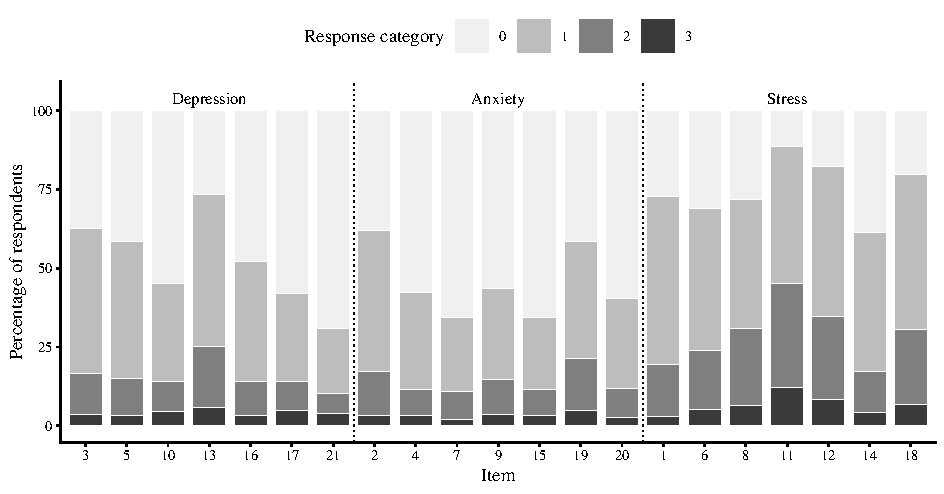
\includegraphics[width=\textwidth]{../figures/fig_distributions.pdf}
\caption{Response distributions of the 21 items, grouped by subscale.}
\label{fig:dist}
\end{figure}

\subsection{Classical test theory}\label{sec:ctt}

Internal consistency is high at every level (Table~\ref{tab:ctt}): $\alpha=\AlphaTotal$
[\AlphaTotalLo, \AlphaTotalHi] for the total scale and \AlphaAnxiety--\AlphaDepression{}
for the subscales. Corrected item--total correlations range from \CITmin{}
(\itemno{2}, ``dryness of the mouth'') to \CITmax{} (\itemno{13}, ``down-hearted and
blue''), and no item would raise $\alpha$ if removed.

What does this license? Not the claim that the DASS-21 measures one thing well.
$\alpha$ depends only on the number of items and their average correlation
($\bar r=\AvgInterItemR$), so with 21 items a modest average correlation is enough for a
large coefficient, whether the items share one factor or several correlated ones. It
also equals reliability only under essential $\tau$-equivalence, which is untenable
here: loadings in the one-factor CFA range from \LoadMin{} to \LoadMax. What $\alpha$
does support -- conservatively, since it is a lower bound -- is that the total score's
standard error of measurement is small ($SEM=\SEMTotal$ points on the 0--63 scale).

The subscale correlations raise a different question. The sums correlate at
$r=\rSubDA$ (D--A), $\rSubDS$ (D--S) and $\rSubAS$ (A--S), and $\rDisAD$, $\rDisDS$
and $\rDisASX$ after correction for attenuation. Constructs that correlate around .8
once measurement error is removed are not ``maximally differentiated'' -- the problem the
DASS was designed to solve, and one reported repeatedly for the short form
\citep{henry2005short}. CTT can raise this question
but not answer it, because it cannot separate a general factor from specific ones.

\begin{table}[t]
\centering\small
\caption{CTT summary. $\bar r$ = mean inter-item correlation; $\omega$ = congeneric
reliability from the CFA (latent-response metric); $\omega_{GY}$ = Green--Yang $\omega$
(observed-score metric); $SEM$ = standard error of measurement.}
\label{tab:ctt}
\begin{tabular}{lr rrr r l rr r}
\toprule
Scale & $k$ & $M$ & $SD$ & Skew & $\bar r$ & $\alpha$ [95\% CI] & $\omega$ & $\omega_{GY}$ & $SEM$\\
\midrule
Total & 21 & 17.15 & 11.77 & 0.98 & .45 & .946 [.941, .950] & .964 & .949 & 2.75 \\
Depression & 7 & 5.03 & 4.46 & 1.26 & .56 & .899 [.890, .907] & .935 & .901 & 1.42 \\
Anxiety & 7 & 4.38 & 4.12 & 1.25 & .48 & .864 [.852, .875] & .911 & .870 & 1.52 \\
Stress & 7 & 7.73 & 4.50 & 0.53 & .54 & .891 [.881, .900] & .923 & .894 & 1.49 
\\
\bottomrule
\end{tabular}
\end{table}

\subsection{Binary IRT}\label{sec:irt}

\paragraph{Model choice and fit.} Under rule A the 2PL fits better than the 1PL,
$\chi^2(20)=\LRTA$, $p<.001$; AIC prefers the 2PL (\AICtwoPLA{} vs.\ \AIConePLA), BIC the
1PL (\BIConePLA{} vs.\ \BICtwoPLA). Andersen's test rejects the Rasch model for a median
split of the raw score ($LR=\AndersenLRA$, $df=\AndersenDFA$, $p<.001$) and for gender
($LR=\AndersenGenderLRA$, $p<.001$). Item-level Rasch fit is better than these global
tests suggest: infit lies between \InfitMinA{} and \InfitMaxA{} for every item, inside
the conventional $0.7$--$1.3$ band. Outfit is more dispersed (\OutfitMinA--\OutfitMaxA):
\itemno{2} is slightly noisy, and the most frequently endorsed items (11, 12, 13) overfit,
which is what one expects when their slopes are steeper than the common Rasch slope.
The 2PL fits reasonably by limited-information criteria
($M_2$-based RMSEA $=\MtwoRMSEAtwoPLA$, CFI $=\MtwoCFItwoPLA$, SRMSR $=\MtwoSRMSRtwoPLA$),
and \SXtwoMisfitA{} items show $S$-$X^2$ misfit at $p<.05$, none after
Benjamini--Hochberg correction. My reading is that the rejections reflect real slope
heterogeneity, which $N=\NAnalysis$ detects easily; the Rasch model is a usable
description for the purposes here, but a strict Rasch measurement claim would not
survive Andersen's test. I base the substantive interpretation on the 2PL.

\paragraph{Item parameters.} Table~\ref{tab:irtA} and Figure~\ref{fig:icc} give the
parameters. Locations range from $b=\BMinA$ (\itemno{11}, ``getting agitated'') to
$b=\BMaxA$ (\itemno{21}, ``life was meaningless''): a severity hierarchy in which
everyday stress reactions are endorsed at low trait levels and existential hopelessness
only at high ones. Discriminations range from $a=\AMinA$ (\itemno{2}, dry mouth) to
$a=\AMaxA$ (\itemno{13}, down-hearted). The contrast is the clearest illustration of what
a slope means: near its location the endorsement probability of \itemno{13} changes far
faster with $\theta$ than that of \itemno{2}, so \itemno{13} separates neighbouring trait
levels sharply and \itemno{2} hardly at all. A somatic sign such as a dry mouth is a weak
indicator of general negative affect -- a substantive finding, not an estimation problem.

\paragraph{Targeting and information.} On the Rasch scale the items span \BcmlMinA{} to
\BcmlMaxA{} logits, and the mean person location is \MeanPersonLocA{}
(Figure~\ref{fig:wright}). Under rule A test information peaks at
$\theta=\MaxInfoThetaA$ ($I=\MaxInfoA$, $SE=\SEMinA$) and corresponds to a reliability
of at least .80 only for $\theta\in\RelRangeA$; marginal reliability is \MargRelA.
Under rule B the curve moves to the right: a higher peak ($\MaxInfoB$ at
$\theta=\MaxInfoThetaB$) but a narrower useful range ($\RelRangeB$) and lower marginal
reliability (\MargRelB). The cut point therefore does not just rescale the results; it
decides \emph{which part of the continuum the binary test measures well}. Rule A
measures well among people with mild symptoms, rule B among people with pronounced
symptoms and hardly at all below the mean.

\paragraph{Comparison with CTT.} The 2PL location and CTT easiness are almost the same
information ($r=\CorrBPA$). Discrimination agrees much less: under rule A, $a$
correlates only $r=\CorrARpbA$ with the corrected item--total correlation of the binary
items, under rule B $r=\CorrARpbB$. The difference is instructive: the point-biserial
correlation depends on item difficulty as well as on discrimination, so when difficulties
are spread widely (rule A) it no longer tracks $a$; when they are concentrated (rule B) it
does. Person estimates and binary sum scores correlate $r=\ThetaSumA$, so IRT does not
\emph{reorder} respondents here; what it adds is an account of how precisely each one is
located, which varies across $\theta$ and which CTT cannot provide.

\begin{table}[t]
\centering\small
\caption{Item parameters under rule A ($0$ vs.\ $1$--$3$). $b_{\text{CML}}$ = Rasch
location (conditional ML); infit/outfit = mean-square fit; $a$, $b$ = 2PL discrimination
and location with standard errors.}
\label{tab:irtA}
\begin{tabular}{ll r rr rr rr rr}
\toprule
Item & Sub & $p$ & $b_{\text{CML}}$ & $SE$ & Infit & Outfit & $a$ & $SE$ & $b$ & $SE$\\
\midrule
3 & D & .63 & $-$0.27 & 0.07 & 0.96 & 0.99 & 1.96 & 0.14 & $-$0.43 & 0.05 \\
5 & D & .58 & 0.01 & 0.07 & 1.07 & 1.11 & 1.63 & 0.12 & $-$0.31 & 0.05 \\
10 & D & .45 & 0.87 & 0.07 & 1.00 & 1.02 & 1.88 & 0.13 & 0.16 & 0.05 \\
13 & D & .73 & $-$1.05 & 0.08 & 0.84 & 0.63 & 2.70 & 0.21 & $-$0.74 & 0.05 \\
16 & D & .52 & 0.42 & 0.07 & 0.94 & 0.88 & 2.12 & 0.15 & $-$0.07 & 0.05 \\
17 & D & .42 & 1.06 & 0.07 & 1.00 & 1.07 & 1.89 & 0.13 & 0.27 & 0.05 \\
21 & D & .31 & 1.84 & 0.08 & 0.96 & 1.02 & 2.01 & 0.15 & 0.65 & 0.05 \\
2 & A & .62 & $-$0.23 & 0.07 & 1.14 & 1.39 & 1.42 & 0.11 & $-$0.48 & 0.06 \\
4 & A & .42 & 1.04 & 0.07 & 1.01 & 1.05 & 1.80 & 0.13 & 0.26 & 0.05 \\
7 & A & .35 & 1.57 & 0.08 & 1.00 & 0.90 & 1.86 & 0.13 & 0.54 & 0.05 \\
9 & A & .44 & 0.96 & 0.07 & 0.89 & 0.84 & 2.28 & 0.16 & 0.19 & 0.05 \\
15 & A & .34 & 1.58 & 0.08 & 1.00 & 1.09 & 1.87 & 0.13 & 0.54 & 0.05 \\
19 & A & .59 & $-$0.00 & 0.07 & 1.07 & 1.19 & 1.62 & 0.12 & $-$0.31 & 0.05 \\
20 & A & .41 & 1.16 & 0.07 & 0.93 & 0.85 & 2.11 & 0.15 & 0.30 & 0.05 \\
1 & S & .73 & $-$1.01 & 0.08 & 0.98 & 1.11 & 1.88 & 0.14 & $-$0.82 & 0.06 \\
6 & S & .69 & $-$0.71 & 0.08 & 0.98 & 0.93 & 1.90 & 0.14 & $-$0.66 & 0.06 \\
8 & S & .72 & $-$0.94 & 0.08 & 0.96 & 0.96 & 1.96 & 0.14 & $-$0.77 & 0.06 \\
11 & S & .89 & $-$2.65 & 0.11 & 0.86 & 0.57 & 2.64 & 0.25 & $-$1.46 & 0.07 \\
12 & S & .82 & $-$1.84 & 0.09 & 0.89 & 0.66 & 2.43 & 0.20 & $-$1.13 & 0.06 \\
14 & S & .61 & $-$0.19 & 0.07 & 0.96 & 0.97 & 2.02 & 0.14 & $-$0.38 & 0.05 \\
18 & S & .80 & $-$1.61 & 0.09 & 1.02 & 0.95 & 1.86 & 0.15 & $-$1.14 & 0.07 
\\
\bottomrule
\end{tabular}
\end{table}

\begin{figure}[t]
\centering
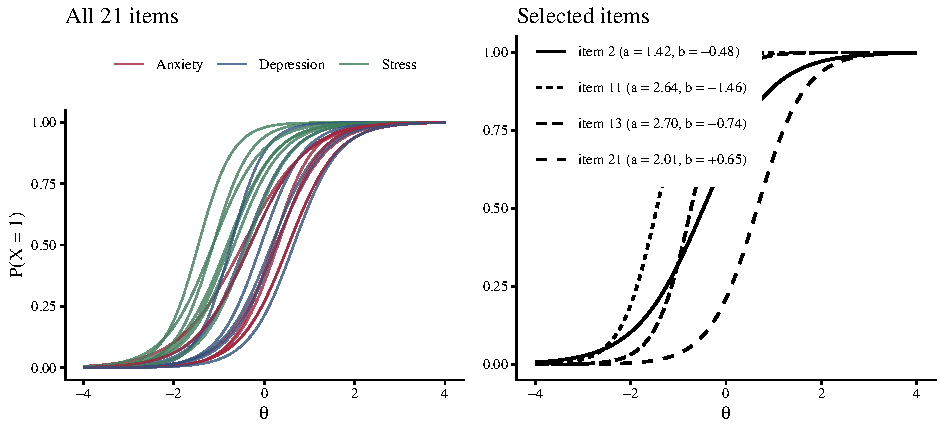
\includegraphics[width=\textwidth]{../figures/fig_icc.pdf}
\caption{2PL item characteristic curves, rule A. Left: all items by subscale. Right:
four items spanning the range of locations and slopes.}
\label{fig:icc}
\end{figure}

\begin{figure}[t]
\centering
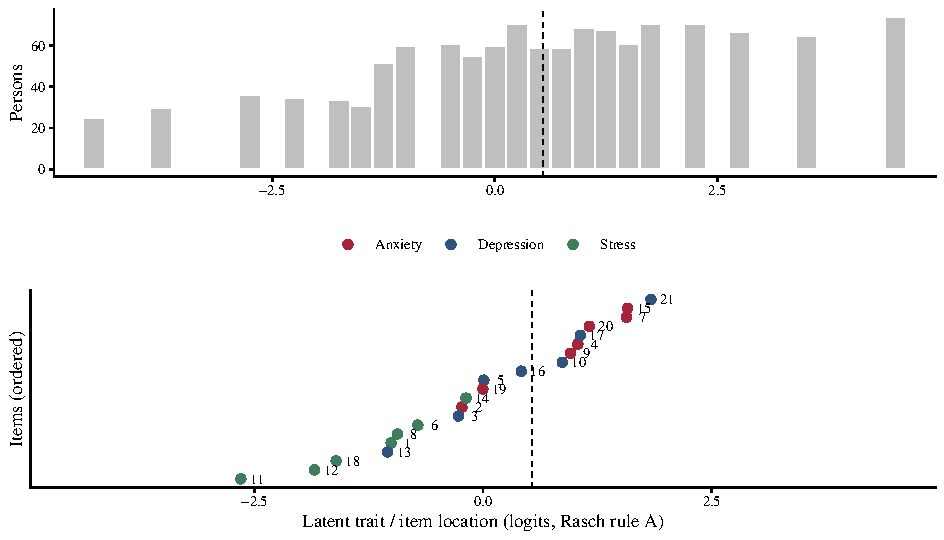
\includegraphics[width=\textwidth]{../figures/fig_wright.pdf}
\caption{Person--item map, Rasch model, rule A. Top: person locations; bottom: item
locations. The dashed line marks the mean person location.}
\label{fig:wright}
\end{figure}

\begin{figure}[t]
\centering
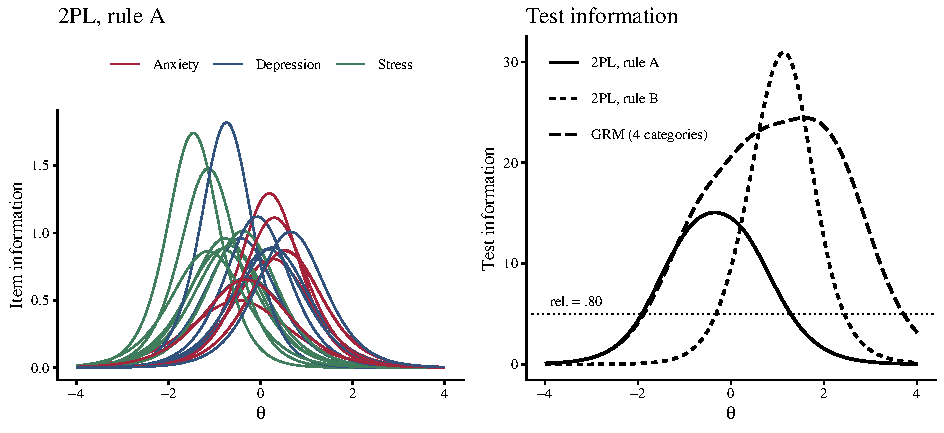
\includegraphics[width=\textwidth]{../figures/fig_information.pdf}
\caption{Left: item information, 2PL rule A. Right: test information of the graded
response model and of the two dichotomised 2PL solutions; the dotted line marks the
information corresponding to a reliability of .80.}
\label{fig:info}
\end{figure}

\subsection{Differential item functioning}\label{sec:dif}

\paragraph{Gender, rule A.} After Benjamini--Hochberg correction the logistic-regression
omnibus test flags \DIFNSig{} items (\DIFSig), Mantel--Haenszel \DIFNSigMH{}
(\DIFSigMH) and Lord's test \DIFNSigLord{} (full results in Table~\ref{tab:dif},
appendix; Figure~\ref{fig:dif}). The effects run in \emph{both} directions. At the same
total score, Group~2 endorses items \DIFFocalMore{} more often: breathing difficulty,
being close to panic, awareness of the heart, feeling scared without reason, and
feeling worthless. Group~1 endorses items \DIFRefMore{} more often: dry mouth, nervous
energy, being intolerant of interruptions, being unable to become enthusiastic, and (only
on the omnibus test, with a negligible effect) life feeling meaningless. No item shows
non-uniform DIF.

Is any of this practically important? The effect sizes say no. \ETSA{} items are ETS
class~A, \ETSB{} class~B and \ETSC{} class~C (\itemno{\MaxDeltaMHItem},
$\Delta_{MH}=\MaxDeltaMH$); the largest $\Delta R^2$ is \MaxdRtwo{}, far below the .035
needed for even a moderate effect, so all 21 items are negligible on the Zumbo--Thomas
criterion. Two further points weaken any claim of bias. Because the effects point in
opposite directions they largely cancel in the total score. And matching on a total that
contains the studied items forces DIF to balance to some extent, so part of the
two-sided pattern may be methodological. The content reading -- panic and cardiorespiratory
symptoms more readily reported by Group~2, low-arousal tension and anhedonia by Group~1 --
is a hypothesis about symptom expression or reporting style, not something these data
can establish. I retain all items and flag them; deleting items on statistical
significance alone at $N>1200$ would be exactly the error the lecture warns against.

\paragraph{Sensitivity to the cut point.} Under rule B, \DIFNSigB{} items are flagged
(\DIFSigB) and \ETSCNB{} reach class~C (\ETSCB); only items \DIFOverlapAB{} are flagged
under both rules. DIF conclusions are therefore \emph{not} invariant to the
dichotomisation: collapsing categories differently changes which region of the
continuum each binary item is sensitive to, and with it where group differences in
endorsement become visible.

\paragraph{Bonus: age and education (exploratory).} Age produces stronger DIF than
gender: \DIFAgeN{} items are significant, class~C effects appear for items
\DIFAgeETSC, and the largest $\Delta R^2$ is \DIFAgeMaxdR. Younger respondents endorse
trembling, worry about panicking in public and agitation (items 7, 9, 11) more at equal
total score, older respondents the inability to become enthusiastic (\itemno{16}) --
social-evaluative and arousal symptoms as markers of distress in the young, anhedonia
in the old. With age as a continuous covariate \DIFAgeContN{} items are flagged,
including all items flagged by the median split, so the result is not an artefact of
the split. Education shows no DIF at all (\DIFEduN{} items with the median split,
\DIFEduContN{} as a continuous covariate, largest $\Delta R^2=\DIFEduMaxdR$). This null
result matters: it shows that the procedures do not flag items indiscriminately at this
sample size.

\begin{figure}[t]
\centering
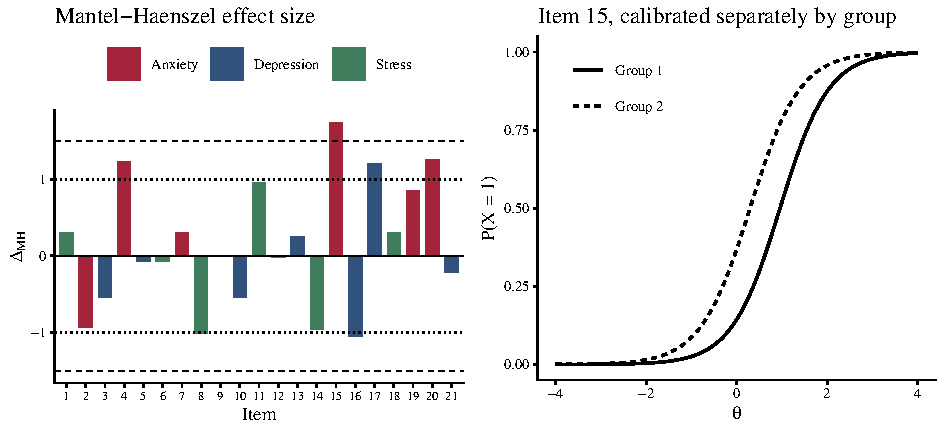
\includegraphics[width=\textwidth]{../figures/fig_dif.pdf}
\caption{Left: Mantel--Haenszel effect sizes by item (gender, rule A); dotted and dashed
lines mark $|\Delta_{MH}|=1$ and $1.5$. Right: item characteristic curves of the item with
the largest effect, calibrated separately in each group.}
\label{fig:dif}
\end{figure}

\subsection{Confirmatory factor analysis}\label{sec:cfa}

Table~\ref{tab:cfafit} reports the four models. The one-factor model is clearly
rejected (CFI $=\CFIOne$, TLI $=\TLIOne$, RMSEA $=\RMSEAOne$, SRMR $=\SRMROne$). The
correlated three-factor model is acceptable by CFI/TLI and SRMR (\CFIThree, \TLIThree,
\SRMRThree) but its RMSEA of \RMSEAThree{} is above the .06 benchmark. The bifactor model
fits best (CFI $=\CFIBi$, RMSEA $=\RMSEABi$, SRMR $=\SRMRBi$), but even it does not reach
close fit on every index, and lavaan's robust indices are less favourable still
(bifactor robust CFI $=\CFIrobBi$, RMSEA $=\RMSEArobBi$), although they rank the models
in the same order. No model reproduces the polychoric correlations exactly; the
comparison is between degrees of approximation. M3 reproduces M2's fit, as it must; its
second-order loadings are \SecondOrderDep{} (Depression), \SecondOrderAnx{} (Anxiety)
and \SecondOrderStr{} (Stress), so nearly all reliable variance in each subscale factor
is shared with one higher-order factor.

That the bifactor model fits best is close to uninformative in itself: it has 18 more
parameters than M2, and bifactor models win such comparisons almost by construction
\citep{reise2013multidimensionality}. The informative results are elsewhere.
\emph{First}, the latent correlations in M2 are very high ($\varphi_{DA}=\PhiDA$,
$\varphi_{DS}=\PhiDS$, $\varphi_{AS}=\PhiAS$). \emph{Second}, in M4 the general loadings
are uniformly strong (\GenLoadMin--\GenLoadMax) while the specific loadings are weak and
uneven (\SpecLoadMin--\SpecLoadMax; Figure~\ref{fig:bifactor}): \itemno{14}
($\lambda_S=\SpecLoadItemFourteen$) and \itemno{5} ($\SpecLoadItemFive$) are pure
indicators of the general factor, whereas \itemno{21} ($\SpecLoadItemTwentyone$),
\itemno{10} ($\SpecLoadItemTen$) and \itemno{4} ($\SpecLoadItemFour$) -- hopelessness
and anhedonia on one side, breathlessness on the other -- carry the clearest specific
variance, exactly the depression/somatic-anxiety contrast the DASS was built on.
\emph{Third}, local dependence largely disappears in M4 (Figure~\ref{fig:resid}): the
largest residual correlations of M1 are between items \ResidPairOne{}
(\ResidValOne), \ResidPairTwo{} (\ResidValTwo) and \ResidPairThree{} (\ResidValThree),
whereas no residual of M4 exceeds \ResidMaxBi{} in absolute value. The specific factors
thus mostly absorb overlap between near-paraphrases within a subscale (breathlessness and
panic; a racing heart and unexplained fear); whether that is a substantive dimension or
shared wording is a judgement the model cannot make.

\begin{table}[t]
\centering\small
\caption{Fit of the measurement models (WLSMV, $N=\NAnalysis$; scaled indices).
\textsuperscript{a}Statistically equivalent to M2 with three first-order factors.}
\label{tab:cfafit}
\begin{tabular}{lrr r rr l r}
\toprule
Model & $q$ & $\chi^{2}$ & $df$ & CFI & TLI & RMSEA [90\% CI] & SRMR\\
\midrule
M1. Unidimensional & 84 & 2663.9 & 189 & .924 & .916 & .104 [.100, .107] & .065 \\
M2. Correlated three-factor & 87 & 1168.6 & 186 & .970 & .966 & .066 [.062, .070] & .040 \\
M3. Second-order\textsuperscript{a} & 87 & 1168.6 & 186 & .970 & .966 & .066 [.062, .070] & .040 \\
M4. Bifactor & 105 & 823.9 & 168 & .980 & .975 & .057 [.053, .061] & .032 
\\
\bottomrule
\end{tabular}
\end{table}

\begin{figure}[t]
\centering
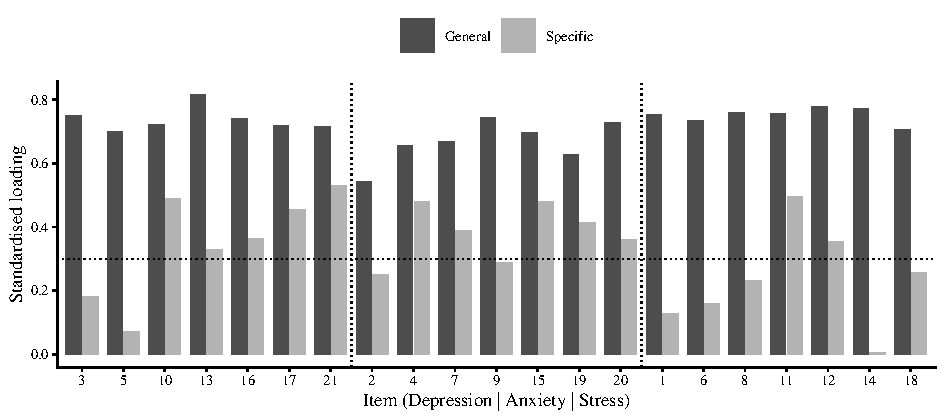
\includegraphics[width=\textwidth]{../figures/fig_bifactor.pdf}
\caption{Standardised loadings in the bifactor model. Dotted line: $\lambda=.30$.}
\label{fig:bifactor}
\end{figure}

\begin{figure}[t]
\centering
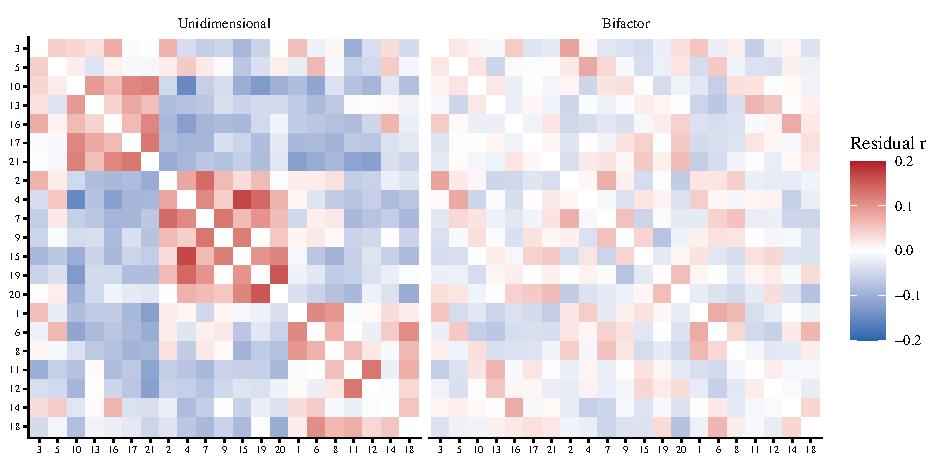
\includegraphics[width=\textwidth]{../figures/fig_residuals.pdf}
\caption{Residual polychoric correlations of the one-factor and the bifactor model,
items ordered by subscale. The within-subscale blocks visible on the left are what the
specific factors absorb.}
\label{fig:resid}
\end{figure}

\subsection{Reliability, dimensionality and the comparison of $\omega$ estimates}
\label{sec:reliability}

Table~\ref{tab:dim} collects the indices; they answer the two questions of the
assignment.

\paragraph{Can the total score be used?} Yes. The general factor accounts for
$\omega_H=\OmegaH$ of total-score variance against $\omega_T=\OmegaT$ for all factors,
so \OmegaRatio{} of the reliable variance in the total score is due to the general factor.
ECV $=\ECV$ exceeds the ``good'' benchmark of .70, construct replicability is
$H=\HGeneral$ and factor determinacy \FDGeneral. PUC $=\PUC$ is below .80 -- with 21
items in three blocks of seven it cannot be higher -- which by the lecture's rule means
that bias from treating the scale as unidimensional is \emph{not} automatically small and
must be judged from the other indices; and these are unambiguous. The total score is a
defensible measure of one general dimension of negative affect.

\paragraph{Can the subscale scores be used?} Much less so. Each subscale is highly
reliable on its own ($\omega=\OmegaDepression$, $\OmegaAnxiety$, $\OmegaStress$), but
almost all of that reliability is borrowed from the general factor: once it is partialled
out, the unique reliability is $\omega_S=\OmegaSDepression$ (Depression),
$\OmegaSAnxiety$ (Anxiety) and $\OmegaSStress$ (Stress). Factor determinacies of the
specific factors (\FDDepression, \FDAnxiety, \FDStress) are below the .80--.90 usually
required before factor scores are interpreted, and construct replicability is low
($H=\HSpecDepression$, $\HSpecAnxiety$, $\HSpecStress$). The contrast for Stress --
$\omega=\OmegaStress$ but $\omega_S=\OmegaSStress$ -- is the single most consequential
number in the analysis, and one a conventional CTT report never produces. A Stress score
is a very reliable measurement -- of general negative affect; as a measure of something
specific to stress it retains less than a tenth of its variance. Difference scores
between subscales, or models entering all three as separate predictors, are poorly
supported.

\paragraph{Why the $\omega$ estimates differ.} Table~\ref{tab:omega} lists ten
reliability estimates for the total score. They differ systematically, and each
difference has an interpretation.
\begin{enumerate}[leftmargin=1.6em,itemsep=2pt,topsep=3pt]
\item \emph{Assumed versus estimated loadings.} $\alpha=\AlphaTotal$ is below the
  congeneric $\omega=\OmegaTotalLin$; the gap (\GapAlphaOmega) is what assuming equal
  loadings costs.
\item \emph{Latent versus observed metric.} Ordinal $\alpha$ (\OrdinalAlpha) and the
  linear $\omega$ coefficients describe a sum of the continuous latent responses $Y^*$, a
  score nobody observes. The Green--Yang coefficients describe the observed 0--3 sum and
  are lower ($\omega$: \OmegaTotalGY{} vs.\ \OmegaTotalLin; $\omega_H$: \OmegaHGY{} vs.\
  \OmegaH). As the lecture puts it, the size of this gap (here \GapLinGY{} and
  \GapLinGYH) estimates how far the linearity and normality assumptions are violated --
  modest, given how skewed the items are. \texttt{BifactorIndicesCalculator}, given the
  ordinal model, returns exactly the Green--Yang values ($\omega=\OmegaTGY$,
  $\omega_H=\OmegaHGY$), an independent confirmation of the hand computation.
\item \emph{All common factors versus the general factor.} $\omega_T$ includes the
  specific factors, $\omega_H$ does not. Reporting only $\omega_T$ for a multidimensional
  scale invites attributing all reliable variance to the construct in the scale's title.
\item \emph{Confirmatory versus exploratory general factor.} The Schmid--Leiman
  $\omega_H$ (\OmegaHEFA) is lower than the confirmatory one (\OmegaH) while $\omega_T$
  is the same (\OmegaTEFA{} vs.\ \OmegaT). The confirmatory model forces each item onto one
  specific factor and lets the general factor absorb everything else; the exploratory
  solution derives the general factor from the correlations of oblique group factors and
  allows cross-loadings, assigning more variance to the group factors. The ``true''
  $\omega_H$ is therefore not a single number but depends on how the general factor is
  defined -- the reason the lecture warns that the functions ``can differ''.
\end{enumerate}
Every coefficient in Table~\ref{tab:omega} is correct; they answer different questions
about different scores. For the observed total score, the defensible statements are
$\omega_{GY}\approx\OmegaTotalGY$ for reliability and $\omega_H\approx\OmegaHGY$--\OmegaH{}
for the part attributable to the general factor.

\begin{table}[t]
\centering\small
\caption{Reliability and dimensionality indices (bifactor model unless stated).}
\label{tab:dim}
\begin{tabular}{@{}p{6.9cm} l p{6.2cm}@{}}
\toprule
Index & Value & Interpretation\\
\midrule
$\omega$, unidimensional model (linear) & .964 & sum-score variance due to one common factor (latent-response metric) \\
$\omega$, unidimensional model (Green--Yang) & .949 & same, in the metric of the observed 0--3 scores \\
$\omega_{T}$, bifactor & .970 & variance due to general \emph{and} specific factors \\
$\omega_{H}$, bifactor (linear) & .908 & variance due to the general factor alone \\
$\omega_{H}$, bifactor (Green--Yang) & .888 & same, observed-score metric \\
$\omega_{H}/\omega_{T}$ & .936 & share of reliable variance due to the general factor \\
ECV & .808 & share of common variance explained by the general factor \\
PUC & .70 & share of item correlations not affected by the specific factors \\
Factor determinacy, general & .962 & correlation of factor-score estimates with the factor \\
\quad Depression: $\omega$ / $\omega_{S}$ / FD & .937 / .169 / .815 & subscale total, unique part, determinacy \\
\quad Anxiety: $\omega$ / $\omega_{S}$ / FD & .912 / .224 / .796 & subscale total, unique part, determinacy \\
\quad Stress: $\omega$ / $\omega_{S}$ / FD & .924 / .081 / .737 & subscale total, unique part, determinacy 
\\
\bottomrule
\end{tabular}
\end{table}

\begin{table}[t]
\centering\small
\caption{Ten reliability estimates for the DASS-21 total score.}
\label{tab:omega}
\begin{tabular}{lll}
\toprule
Estimate & Metric & Value\\
\midrule
Cronbach's $\alpha$ (raw item scores) & observed score & .946 \\
Ordinal $\alpha$ (polychoric correlations) & latent response & .962 \\
$\omega$, unidimensional CFA (linear) & latent response & .964 \\
$\omega$, unidimensional CFA (Green--Yang) & observed score & .949 \\
$\omega_{T}$, bifactor CFA (linear) & latent response & .970 \\
$\omega_{T}$, bifactor CFA (Green--Yang) & observed score & .955 \\
$\omega_{H}$, bifactor CFA (linear) & latent response & .908 \\
$\omega_{H}$, bifactor CFA (Green--Yang) & observed score & .888 \\
$\omega_{H}$, EFA + Schmid--Leiman & latent response & .862 \\
$\omega_{T}$, EFA + Schmid--Leiman & latent response & .969 
\\
\bottomrule
\end{tabular}
\end{table}

\subsection{Measurement invariance}\label{sec:mi}

Table~\ref{tab:mi} reports the sequence for the three-factor and the one-factor model.
The configural three-factor model fits acceptably in both groups (CFI $=\MIConfiguralCFI$,
RMSEA $=\MIConfiguralRMSEA$), so the same factor structure holds and the comparison is
meaningful.

\emph{Loadings.} Constraining them is supported by the difference test,
$\Delta\chi^2(\MIMetricddf)=\MIMetricdChi$, $p=\MIMetricdp$, and does not worsen
approximate fit. Metric invariance holds, consistent with the absence of non-uniform DIF:
the items relate to the factors equally strongly in both groups.

\emph{Thresholds.} Here the criteria diverge. Relative to the metric model,
$\Delta\chi^2(\MIScalarddf)=\MIScalardChi$ ($p=\MIScalardp$) and
$\Delta$CFI $=\MIScalardCFI$, $\Delta$RMSEA $=\MIScalardRMSEA$ -- inside the general
$-.010$ criterion but outside Chen's stricter $-.005$ for unequal groups. These
consecutive comparisons are, however, distorted by the scaled-and-shifted statistic,
which is not monotone across nested models: the metric model has a \emph{better} CFI
(\MIMetricCFI) than the less constrained configural model (\MIConfiguralCFI). This is
precisely why the lecture recommends comparing the threshold model directly with the
configural model. That comparison gives $\Delta$CFI $=\MIConfScalardCFI$ and
$\Delta$RMSEA $=\MIConfScalardRMSEA$ -- no deterioration -- while the difference test,
$\Delta\chi^2(\MIConfScalarddf)=\MIConfScalardChi$, $p<.001$, rejects exact equality. I
conclude that thresholds are \emph{approximately} invariant: exact invariance is
rejected, but the misfit it causes is small. Equal residual variances add no meaningful
misfit ($\Delta\chi^2(\MIStrictddf)=\MIStrictdChi$, $p=\MIStrictdp$; $\Delta$CFI
$=\MIStrictdCFI$).

\emph{Where is the non-invariance?} Releasing each item's thresholds in turn,
\PartialNSigBH{} items improve fit significantly after correction, most of all
\itemno{\PartialTopItem} ($\Delta\chi^2=\PartialTopChi$), followed by items
\PartialItems. Items 17, 19 and 15 are also flagged in the DIF analysis, and \itemno{2}
is among the Group-1-favoured DIF items: two different procedures, applied to binary
versus four-category data, point at the same items. Freeing the thresholds of the four
worst items changes the latent mean differences only slightly (Depression \KappaDepression{}
$\rightarrow$ \KappaPartialDepression, Anxiety \KappaAnxiety{} $\rightarrow$
\KappaPartialAnxiety, Stress \KappaStress{} $\rightarrow$ \KappaPartialStress{} SD).

\emph{What may be compared?} The factor structure and the loadings are comparable
across groups, and latent means can be compared with the caveat of approximate threshold
invariance: Group~2 is higher by \KappaDepression{} (Depression), \KappaAnxiety{} (Anxiety)
and \KappaStress{} (Stress) SD, and by \KappaUni{} SD on the single general factor. Whether
\emph{observed sum scores} may be compared is a separate question, since sum-score bias
depends on whether threshold differences cancel or accumulate across items. Here they
largely cancel: the standardised differences of the observed subscale sums
($\DGenderDep$, $\DGenderAnx$, $\DGenderStr$) are close to the latent differences under
both the full and the partial model. The one-factor model shows the same pattern but its
configural fit is poor (CFI $=\MIUConfiguralCFI$, RMSEA $=\MIUConfiguralRMSEA$), so its
invariance tests describe a model that does not fit well to begin with.

\paragraph{Bonus: age (exploratory).} For the age split (Table~\ref{tab:miage},
appendix) loadings are again invariant ($p=\MIAgeMetricdp$), but the threshold step fails
both consecutive criteria (Metric $\rightarrow$ scalar: $\Delta$CFI
$=\MIAgeScalardCFI$, $p<.001$) and strict invariance is rejected by the difference test
($p=\MIAgeStrictdp$); only the direct configural--scalar comparison
($\Delta$CFI $=\MIAgeConfScalardCFI$) is unproblematic. Older respondents score lower on
all three factors (\KappaAgeDepression, \KappaAgeAnxiety, \KappaAgeStress{} SD). Together
with the stronger age DIF, this means comparisons between age groups rest on a weaker
measurement basis than comparisons between the gender groups.

\begin{table}[t]
\centering\footnotesize
\setlength{\tabcolsep}{4pt}
\caption{Measurement invariance across gender (WLSMV, four-category data, scaled
indices). Metric = equal loadings; scalar = equal loadings and thresholds; strict =
additionally equal residual variances. $\Delta$ columns compare each model with the
previous one; the last row of each block compares scalar with configural directly.}
\label{tab:mi}
\begin{tabular}{ll rr rr rl rr}
\toprule
Model & Step & $\chi^{2}$ & $df$ & CFI & RMSEA & $\Delta\chi^{2}$ ($df$) & $p$ & $\Delta$CFI & $\Delta$RMSEA\\
\midrule
Three-factor & Configural & 1315.4 & 372 & .971 & .065 &  &  &  &  \\
 & Metric & 1046.9 & 390 & .980 & .053 & 27.7 (18) & .068 & +.009 & $-$.012 \\
 & Scalar & 1359.9 & 429 & .971 & .060 & 58.8 (39) & .022 & $-$.008 & +.007 \\
 & Strict & 1167.4 & 450 & .978 & .051 & 30.5 (21) & .083 & +.007 & $-$.009 \\
 & \emph{Scalar vs.\ configural} &  &  &  &  & 134.6 (57) & $<.001$ & +.000 & $-$.005 \\
\addlinespace
One-factor & Configural & 2695.6 & 378 & .928 & .101 &  &  &  &  \\
 & Metric & 1875.3 & 398 & .954 & .078 & 28.3 (20) & .104 & +.026 & $-$.022 \\
 & Scalar & 2539.3 & 439 & .935 & .089 & 53.0 (41) & .099 & $-$.019 & +.011 \\
 & Strict & 2000.8 & 460 & .952 & .074 & 31.1 (21) & .072 & +.017 & $-$.015 \\
 & \emph{Scalar vs.\ configural} &  &  &  &  & 130.7 (61) & $<.001$ & +.007 & $-$.012 
\\
\bottomrule
\end{tabular}
\end{table}

\subsection{Polytomous IRT and the cost of dichotomisation}\label{sec:grm}

The graded response model is the best of the polytomous models by AIC and BIC
(Table~\ref{tab:poly}); it fits clearly better than the GPCM with the same number of
parameters and than the GRM with one common slope ($\Delta\chi^2(20)=\GRMLRT$). The
items therefore differ in how sharply they separate trait levels, and the cumulative
formulation suits these data better than the adjacent-category one. Discriminations
range from \GRMAMin{} (\itemno{2}) to \GRMAMax{} (\itemno{13}) -- the same extremes as in
the binary analysis -- with three ordered boundaries per item (Table~\ref{tab:grm}).

\paragraph{Category functioning.} Because the GRM orders its boundaries by construction,
it cannot show disordered thresholds; the meaningful check is in the divide-by-total
models. In both the PCM and the GPCM all step parameters are ordered
(\DisorderedPCM{} and \DisorderedGPCM{} items with disordered steps), and in all three
models every category is the most probable response somewhere on the continuum
(Figure~\ref{fig:grmcat}). Respondents use the four categories in the intended order, so
there is no empirical reason to collapse them.

\paragraph{Fit.} By limited-information criteria the unidimensional GRM fits only
approximately ($M_2$-based RMSEA $=\GRMMtwoRMSEA$, CFI $=\GRMMtwoCFI$,
SRMSR $=\GRMMtwoSRMSR$), while no item shows $S$-$X^2$ misfit after correction. This
mirrors the CFA: the misfit is not located in single items but in the residual
correlations within subscales that a one-dimensional model cannot reproduce.

\paragraph{Information.} The GRM reaches its maximum information
($\GRMMaxInfo$) at $\theta=\GRMMaxInfoTheta$ and provides a reliability of at least .80
over $\theta\in\GRMRelRange$; its marginal reliability is \GRMMargRel, against
\MargRelA{} (rule A) and \MargRelB{} (rule B). Mean standard errors of the person
estimates are \MeanSEGRM, \MeanSEA{} and \MeanSEB{} respectively: under rule B a
respondent is located with an error \SEratioBGRM{} times as large. Integrated over the
continuum the GRM carries \InfoRatioA{} times the information of the rule-A 2PL and
\InfoRatioB{} times that of rule B (Figure~\ref{fig:info}). This ratio should be read as
precision per unit of a standardised trait, since each model standardises its own
$\theta$; the marginal reliabilities make the same point in a conventional metric.
Rule B is instructive: its \emph{peak} information (\MaxInfoB) is higher than the GRM's,
but over a narrow band at the top of the scale. Dichotomisation does not lose information
uniformly; it concentrates what remains around the cut point.

GRM person estimates correlate \GRMThetaCorrA{} and \GRMThetaCorrB{} with the rule-A and
rule-B estimates and \GRMThetaSum{} with the raw sum: dichotomisation largely preserves
the ranking of respondents and costs precision, especially in the tails. The exercise
required a binary analysis, and it is useful for making the item parameters and the Rasch
fit machinery visible in their simplest form; for measuring individuals with this
instrument, however, the four categories should be kept.

\begin{table}[t]
\centering\small
\caption{Polytomous IRT models. $q$ = number of parameters.}
\label{tab:poly}
\begin{tabular}{lrrrr}
\toprule
Model & $q$ & $\log L$ & AIC & BIC\\
\midrule
GRM & 84 & $-$22019.6 & 44207 & 44636 \\
GRM, common slope & 64 & $-$22126.9 & 44382 & 44708 \\
GPCM & 84 & $-$22063.9 & 44296 & 44724 \\
PCM & 64 & $-$22183.8 & 44496 & 44822 
\\
\bottomrule
\end{tabular}
\end{table}

\begin{table}[t]
\centering\small
\caption{Graded response model parameters. $b_1$--$b_3$ = category boundaries;
spread = $b_3-b_1$; $I_{\max}$ = maximum item information.}
\label{tab:grm}
\begin{tabular}{ll r rrr r r}
\toprule
Item & Sub & $a$ & $b_1$ & $b_2$ & $b_3$ & Spread & $I_{\max}$\\
\midrule
3 & D & 2.16 & $-$0.41 & 1.19 & 2.37 & 2.78 & 1.28 \\
5 & D & 1.73 & $-$0.31 & 1.39 & 2.73 & 3.04 & 0.84 \\
10 & D & 2.27 & 0.13 & 1.29 & 2.17 & 2.04 & 1.50 \\
13 & D & 2.87 & $-$0.71 & 0.74 & 1.85 & 2.56 & 2.16 \\
16 & D & 2.25 & $-$0.08 & 1.31 & 2.39 & 2.46 & 1.41 \\
17 & D & 2.18 & 0.23 & 1.33 & 2.17 & 1.94 & 1.40 \\
21 & D & 2.26 & 0.59 & 1.55 & 2.28 & 1.68 & 1.53 \\
2 & A & 1.24 & $-$0.52 & 1.56 & 3.24 & 3.76 & 0.44 \\
4 & A & 1.71 & 0.24 & 1.64 & 2.75 & 2.51 & 0.86 \\
7 & A & 1.71 & 0.53 & 1.71 & 3.03 & 2.51 & 0.86 \\
9 & A & 2.12 & 0.18 & 1.29 & 2.37 & 2.20 & 1.29 \\
15 & A & 1.95 & 0.49 & 1.53 & 2.58 & 2.08 & 1.12 \\
19 & A & 1.58 & $-$0.34 & 1.10 & 2.51 & 2.85 & 0.72 \\
20 & A & 2.03 & 0.28 & 1.49 & 2.63 & 2.35 & 1.17 \\
1 & S & 2.03 & $-$0.79 & 1.08 & 2.56 & 3.35 & 1.10 \\
6 & S & 1.92 & $-$0.66 & 0.91 & 2.24 & 2.90 & 1.02 \\
8 & S & 2.12 & $-$0.74 & 0.61 & 1.99 & 2.73 & 1.23 \\
11 & S & 2.27 & $-$1.50 & 0.15 & 1.46 & 2.96 & 1.38 \\
12 & S & 2.38 & $-$1.12 & 0.47 & 1.71 & 2.83 & 1.51 \\
14 & S & 2.06 & $-$0.38 & 1.19 & 2.32 & 2.70 & 1.18 \\
18 & S & 1.87 & $-$1.12 & 0.65 & 2.06 & 3.18 & 0.96 
\\
\bottomrule
\end{tabular}
\end{table}

\begin{figure}[t]
\centering
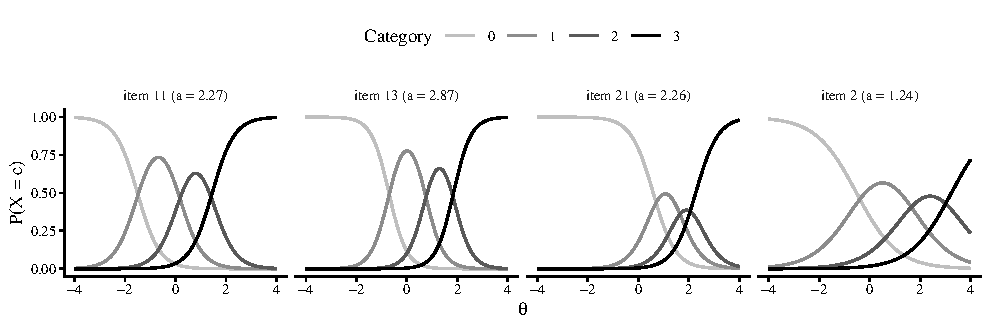
\includegraphics[width=\textwidth]{../figures/fig_grm_cat.pdf}
\caption{GRM category response curves for four items spanning the range of
discriminations. Every category is the most probable response over some region of
$\theta$.}
\label{fig:grmcat}
\end{figure}

%==============================================================================
\section{Integrated Discussion}\label{sec:integration}
%==============================================================================

All analyses were run on the same respondents so that they can be compared directly.

\subsection{Where the methods agree}

\paragraph{Ordering of persons.} Sum scores, 2PL and GRM person estimates rank
respondents almost identically ($r=\ThetaSumA$ between the 2PL estimate and the binary
sum, $r=\GRMThetaSum$ between the GRM estimate and the raw sum). If the only aim is to
order people on one continuum, the sophisticated methods do not do it better. What IRT
adds is an account of the \emph{precision} of that ordering, of comparability across
groups, and of the behaviour of individual items.

\paragraph{Ordering and quality of items.} CTT easiness and IRT location carry the same
information ($r=\CorrBPA$). The CFA loadings, transformed into logistic discriminations
by $a_i=1.702\,\lambda_i/\sqrt{1-\lambda_i^2}$ (lecture 6), correlate $\CorrIFAIRT$ with
the 2PL slopes estimated directly from the binary data (Figure~\ref{fig:ifairt},
appendix). Since one set comes from four-category polychoric correlations and the other
from binary responses by marginal maximum likelihood, this is a concrete demonstration
that item factor analysis and IRT are one model in two notations; the remaining scatter
reflects the information lost by dichotomising. \itemno{2} (dry mouth) is the weakest item
and \itemno{13} (down-hearted) the strongest on every criterion: corrected item--total
correlation, CFA loading, 2PL slope and GRM slope.

\paragraph{Dimensionality.} The disattenuated subscale correlations (\rDisAD--\rDisDS),
the latent correlations (\PhiDA--\PhiDS), the second-order loadings
(\SecondOrderAnx--\SecondOrderStr) and the bifactor indices (ECV $=\ECV$,
$\omega_H/\omega_T=\OmegaRatio$) say the same thing from four directions: one strong
general dimension with thin specific residues. Earlier Rasch analyses of the
DASS-21 likewise found that the full scale does not meet strict Rasch requirements as one
measure \citep{shea2009rasch}; the present data agree that a single \emph{strict}
unidimensional model is too restrictive while a general factor clearly dominates.

\paragraph{Gender.} DIF and invariance testing agree that loadings/slopes are equal
(no non-uniform DIF; metric invariance holds), that a few items differ in location
(uniform DIF; threshold non-invariance), that these are largely the same items, and that
the differences are small and partly cancel.

\subsection{Where the methods disagree, and why}

\paragraph{Discrimination in CTT and IRT.} The corrected item--total correlation tracks
the 2PL slope poorly under rule A ($r=\CorrARpbA$) and well under rule B
($r=\CorrARpbB$). The CTT index confounds discrimination with difficulty, so an applied
researcher who deletes the item with the lowest item--total correlation may delete the
item with the most extreme location rather than the least informative one.

\paragraph{Is the scale unidimensional?} The one-factor CFA is rejected (CFI $=\CFIOne$,
RMSEA $=\RMSEAOne$), whereas the bifactor indices say the scale is essentially
unidimensional ($\omega_H=\OmegaH$, ECV $=\ECV$). Both are right because they answer
different questions. The CFA asks whether one factor reproduces the correlations
\emph{exactly}, and at $N=\NAnalysis$ it detects the local dependence within subscales.
The bifactor indices ask how much bias scoring the scale as unidimensional would
introduce: little. Statistical and practical dimensionality are different properties, and
the bifactor framework is valuable precisely because it separates them.

\paragraph{Are the thresholds invariant?} Difference tests reject exact equality, the
direct configural--scalar $\Delta$CFI shows no deterioration, consecutive $\Delta$CFI
values are inflated or deflated by the non-monotone scaled statistic, and the DIF effect
sizes are negligible. These are not contradictions but answers to different questions:
significance tests ask whether differences are exactly zero (they are not), fit and effect
size criteria ask whether they are large enough to matter (they are not). Reporting only
one of them would misrepresent the data.

\paragraph{Do the binary and polytomous analyses agree?} On the ordering of items and
persons, yes; on precision, no (Section~\ref{sec:grm}); and on DIF only partly, since the
flagged items depend on the cut point. Dichotomisation is not a neutral preprocessing step,
even for questions that seem far removed from it.

\subsection{What each framework contributed}

\emph{CTT alone} would have reported $\alpha=\AlphaTotal$ and three reliable subscales and
concluded that the DASS-21 works well -- missing that the subscales are barely separable
and that precision is lowest where many respondents are. \emph{IRT} revealed targeting,
conditional precision and the item hierarchy, but a unidimensional model cannot ask
whether three dimensions exist. \emph{CFA} established the structure and the misfit of the
one-factor model but says nothing about where on the continuum the scale measures well.
\emph{The bifactor model} answered the scoring question none of the others can pose.
\emph{DIF and invariance testing} were needed before any group comparison could be
interpreted. \emph{The polytomous model} showed what the binary analysis cost. The methods
are not competing answers to one question; they answer different questions that a
complete evaluation of an instrument has to ask.

%==============================================================================
\section{Limitations}\label{sec:limitations}
%==============================================================================

\emph{Design.} The data are cross-sectional, from one non-clinical population, without
an external criterion, clinical diagnosis or retest. Nothing here speaks to criterion
validity or test--retest reliability, or to whether the same general factor would emerge
in a clinical sample, where symptom profiles rather than overall severity may vary more.

\emph{Coding and content.} Without a codebook the gender labels are an inference
(Section~\ref{sec:sample}); the content interpretation of the DIF pattern would reverse if
the labels did. The content interpretations also assume the published English item
wording; the data contain no item text.

\emph{Model fit.} No model fits exactly, and the conclusions rest on approximate fit. The
choice between scaled and robust fit indices matters for absolute judgements (the robust
indices are less favourable) though not for the ranking of models. Every IRT model
fitted assumes local independence, which the residual correlations within subscales
mildly violate; this slightly inflates slopes and reliability for the affected items.

\emph{Bifactor interpretation.} The bifactor model fits better partly because it is more
flexible, and bifactor solutions are sample-dependent
\citep{reise2013multidimensionality}; its superior fit is not evidence of a bifactor
\emph{process}. The conclusions rest on the loading pattern and the reliability
decomposition, and the Schmid--Leiman $\omega_H$ (\OmegaHEFA) shows that the size of the
general factor depends on how it is defined.

\emph{DIF and invariance.} The DIF procedures match on an observed score that contains
the studied items, which can create spurious balancing effects; purification mitigates but
does not remove this. The multi-group models are large relative to the smaller group
($n=\NAnalysisGroupOne$), the $\Delta$CFI cut-offs were derived for continuous indicators,
and the age and education analyses use median splits (although the continuous-covariate
check reproduces the age result). The bonus analyses are exploratory.

\emph{What cannot be concluded.} These data do not show that the subscales are invalid,
only that in this sample their unique reliable variance is small. They do not show that
any item is biased in a way that warrants removal, only that some function slightly
differently. And they cannot settle whether a general factor of negative affect is a
psychological entity or a convenient summary; a factor analysis of one questionnaire has
nothing decisive to say about that.

%==============================================================================
\section{Conclusion}\label{sec:conclusion}
%==============================================================================

In this sample the DASS-21 is a reliable measure of one broad dimension of negative
affect. A total score is defensible: the general factor accounts for \OmegaRatio{} of its
reliable variance (ECV $=\ECV$). Separate subscale scores are much harder to justify,
because after the general factor is partialled out they retain only
$\omega_S=\OmegaSStress$--\OmegaSAnxiety{} of unique reliable variance and their factor
scores are not determinate enough to interpret -- a limit that remains invisible in a
conventional CTT report. Measurement across the two gender groups is comparable for
practical purposes: loadings are invariant, thresholds approximately so, the items with
differential functioning have negligible effects in both directions, and latent mean
differences barely change when the least invariant items are freed. Age is a stronger
source of differential functioning than gender, education none at all.

The most instructive result is methodological. Dichotomising the four-category items --
required by the exercise and common in practice -- costs much of the test information,
moves the region in which the instrument measures well, and changes which items appear
biased. Running the binary analysis under two rules and against the graded model was
more informative than running it once.

%==============================================================================
\section*{Use of AI Assistance}
\addcontentsline{toc}{section}{Use of AI Assistance}
%==============================================================================

As requested in the assignment, I declare that I used an AI assistant (Claude,
Anthropic) for this essay: for writing and debugging the R code of the analysis reports
and for drafting and editing the text. I ran all analyses myself, checked the
methodological choices against the course material, and am responsible for the
interpretations. All numbers in the text and tables are generated by the R code from
the data.

\printbibliography[heading=bibnumbered,title={References}]

%==============================================================================
\appendix
\section{Supplementary Tables and Figures}
%==============================================================================

\begin{table}[h]
\centering\small
\caption{Item parameters under rule B ($0$--$1$ vs.\ $2$--$3$), sensitivity analysis.}
\label{tab:irtB}
\begin{tabular}{ll r r rr rr}
\toprule
Item & Sub & $p$ & $b_{\text{CML}}$ & Infit & Outfit & $a$ (2PL) & $b$ (2PL)\\
\midrule
3 & D & .16 & 0.24 & 0.90 & 0.90 & 2.86 & 1.15 \\
5 & D & .15 & 0.40 & 1.05 & 1.12 & 2.16 & 1.32 \\
10 & D & .14 & 0.53 & 0.88 & 0.79 & 3.10 & 1.23 \\
13 & D & .25 & $-$0.65 & 0.83 & 0.72 & 3.66 & 0.77 \\
16 & D & .14 & 0.54 & 0.91 & 0.92 & 2.84 & 1.26 \\
17 & D & .14 & 0.53 & 0.87 & 0.84 & 3.20 & 1.22 \\
21 & D & .10 & 1.07 & 0.90 & 0.84 & 2.94 & 1.45 \\
2 & A & .17 & 0.16 & 1.35 & 1.79 & 1.42 & 1.48 \\
4 & A & .12 & 0.87 & 1.02 & 1.09 & 2.23 & 1.50 \\
7 & A & .11 & 1.01 & 1.00 & 1.12 & 2.24 & 1.56 \\
9 & A & .15 & 0.47 & 0.94 & 0.84 & 2.68 & 1.26 \\
15 & A & .12 & 0.88 & 0.90 & 0.78 & 2.82 & 1.39 \\
19 & A & .21 & $-$0.30 & 1.12 & 1.18 & 2.06 & 1.04 \\
20 & A & .12 & 0.86 & 0.93 & 0.61 & 2.91 & 1.37 \\
1 & S & .19 & $-$0.08 & 0.95 & 0.85 & 2.69 & 1.04 \\
6 & S & .24 & $-$0.54 & 1.04 & 1.06 & 2.27 & 0.91 \\
8 & S & .31 & $-$1.16 & 0.98 & 0.94 & 2.60 & 0.63 \\
11 & S & .45 & $-$2.36 & 0.98 & 0.87 & 2.86 & 0.17 \\
12 & S & .35 & $-$1.48 & 0.92 & 0.88 & 3.03 & 0.49 \\
14 & S & .17 & 0.16 & 0.99 & 0.98 & 2.49 & 1.16 \\
18 & S & .31 & $-$1.15 & 1.09 & 1.26 & 2.20 & 0.66 
\\
\bottomrule
\end{tabular}
\end{table}

\begin{table}[h]
\centering\small
\caption{DIF with respect to gender, rule A. $\Delta_{MH}$ = ETS delta (positive: Group~2
endorses more at equal total score); ETS = A/B/C class; $LR_u$, $LR_{nu}$ = uniform and
non-uniform likelihood-ratio statistics; $\Delta R^2$ = Nagelkerke effect size with
Zumbo--Thomas class; $\chi^2_L$ = Lord's statistic.
$^{*}p<.05$, $^{**}p<.01$, $^{***}p<.001$ (unadjusted).}
\label{tab:dif}
\begin{tabular}{ll rr l rr rl r}
\toprule
Item & Sub & $\chi^{2}_{MH}$ & $\Delta_{MH}$ & ETS & $LR_u$ & $LR_{nu}$ & $\Delta R^{2}$ & Z--T & $\chi^{2}_{L}$\\
\midrule
3 & D & 1.74 & $-$0.54 & A & 2.33 & 0.35 & .002 & A & 2.18 \\
5 & D & 0.02 & $-$0.07 & A & 0.20 & 1.92 & .000 & A & 2.99 \\
10 & D & 1.74 & $-$0.54 & A & 2.34 & 0.18 & .002 & A & 3.02 \\
13 & D & 0.23 & 0.25 & A & 0.24 & 1.01 & .001 & A & 1.10 \\
16 & D & 7.33$^{**}$ & $-$1.05 & B & 8.94$^{**}$ & 0.43 & .007 & A & 7.03$^{*}$ \\
17 & D & 9.35$^{**}$ & 1.20 & B & 9.65$^{**}$ & 0.03 & .007 & A & 3.09 \\
21 & D & 0.21 & $-$0.22 & A & 0.13 & 3.16 & .008 & A & 2.60 \\
2 & A & 6.50$^{*}$ & $-$0.93 & A & 7.81$^{**}$ & 0.02 & .007 & A & 6.21$^{*}$ \\
4 & A & 10.69$^{**}$ & 1.23 & B & 11.85$^{***}$ & 0.01 & .008 & A & 4.80 \\
7 & A & 0.49 & 0.30 & A & 0.56 & 2.14 & .002 & A & 3.92 \\
9 & A & 0.00 & 0.01 & A & 0.04 & 0.72 & .000 & A & 2.53 \\
15 & A & 18.84$^{***}$ & 1.74 & C & 19.66$^{***}$ & 0.10 & .014 & A & 8.13$^{*}$ \\
19 & A & 5.88$^{*}$ & 0.85 & A & 6.41$^{*}$ & 1.45 & .006 & A & 3.74 \\
20 & A & 10.10$^{**}$ & 1.26 & B & 9.22$^{**}$ & 0.52 & .007 & A & 2.58 \\
1 & S & 0.47 & 0.31 & A & 0.46 & 0.59 & .003 & A & 0.59 \\
6 & S & 0.01 & $-$0.07 & A & 0.07 & 0.93 & .000 & A & 1.46 \\
8 & S & 5.22$^{*}$ & $-$1.01 & B & 6.54$^{*}$ & 1.52 & .006 & A & 5.01 \\
11 & S & 2.35 & 0.96 & A & 2.17 & 0.00 & .003 & A & 1.39 \\
12 & S & 0.00 & $-$0.02 & A & 0.10 & 0.37 & .001 & A & 0.20 \\
14 & S & 5.75$^{*}$ & $-$0.97 & A & 7.44$^{**}$ & 0.34 & .005 & A & 5.32 \\
18 & S & 0.37 & 0.30 & A & 0.50 & 2.73 & .003 & A & 2.85 
\\
\bottomrule
\end{tabular}
\end{table}

\begin{table}[h]
\centering\footnotesize
\setlength{\tabcolsep}{4pt}
\caption{Measurement invariance across age groups (bonus analysis; layout as
Table~\ref{tab:mi}).}
\label{tab:miage}
\begin{tabular}{ll rr rr rl rr}
\toprule
Model & Step & $\chi^{2}$ & $df$ & CFI & RMSEA & $\Delta\chi^{2}$ ($df$) & $p$ & $\Delta$CFI & $\Delta$RMSEA\\
\midrule
Three-factor & Configural & 1395.8 & 372 & .969 & .067 &  &  &  &  \\
 & Metric & 1075.8 & 390 & .980 & .054 & 15.7 (18) & .616 & +.010 & $-$.014 \\
 & Scalar & 1476.8 & 429 & .969 & .064 & 152.2 (39) & $<.001$ & $-$.011 & +.010 \\
 & Strict & 1293.5 & 450 & .975 & .056 & 44.3 (21) & .002 & +.006 & $-$.008 \\
 & \emph{Scalar vs.\ configural} &  &  &  &  & 161.5 (57) & $<.001$ & $-$.001 & $-$.004 \\
\addlinespace
One-factor & Configural & 2822.2 & 378 & .927 & .103 &  &  &  &  \\
 & Metric & 1999.5 & 398 & .952 & .082 & 42.8 (20) & .002 & +.025 & $-$.022 \\
 & Scalar & 2696.9 & 439 & .933 & .092 & 15.2 (41) & 1.000 & $-$.020 & +.011 \\
 & Strict & 2203.3 & 460 & .948 & .079 & 69.6 (21) & $<.001$ & +.015 & $-$.013 \\
 & \emph{Scalar vs.\ configural} &  &  &  &  & 158.8 (61) & $<.001$ & +.006 & $-$.011 
\\
\bottomrule
\end{tabular}
\end{table}

\begin{figure}[h]
\centering
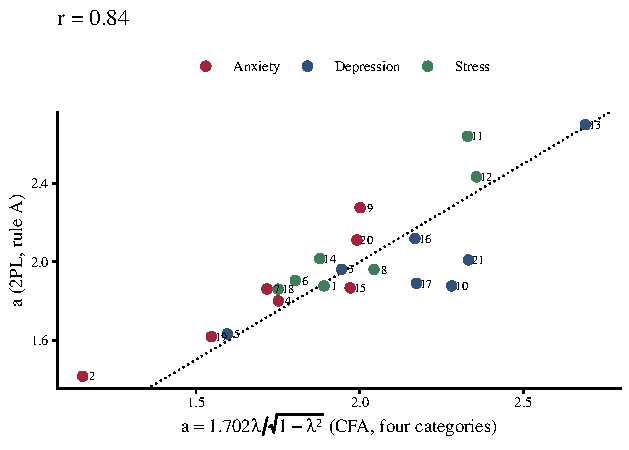
\includegraphics[width=.62\textwidth]{../figures/fig_ifa_irt.pdf}
\caption{Discriminations implied by the one-factor CFA loadings versus 2PL
discriminations estimated from the rule-A data.}
\label{fig:ifairt}
\end{figure}

\begin{figure}[h]
\centering
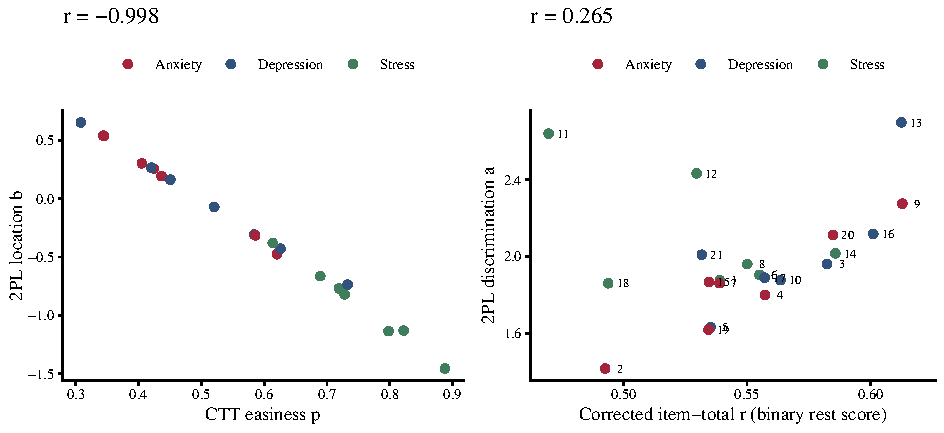
\includegraphics[width=\textwidth]{../figures/fig_ctt_irt.pdf}
\caption{CTT and IRT item indices, rule A.}
\label{fig:cttirt}
\end{figure}

\section{Reproducing the Analysis}

The project folder contains the raw data (folder \texttt{data}), ten R~Markdown
reports numbered 00 to 09 (folder \texttt{analysis}), a shared setup file (folder
\texttt{R}) and this document (folder \texttt{essay}). Running the script
\texttt{run\_all.R} from the project folder renders all reports in order. The last
report writes the tables, the figures and the macro file \texttt{numbers.tex} from which
the numbers in the text are taken, so recompiling this document afterwards reproduces
the essay from the data.

\end{document}
